% In questo file vengono definiti comandi (macro) utili in tutti i documenti

\newcommand{\gruppo}{\textit{Sirius}} % nome gruppo
\newcommand{\progetto}{\textit{Sequenziatore}} % nome progetto
\newcommand{\capitolato}{\href{http://www.math.unipd.it/~tullio/IS-1/2013/Progetto/C4p.pdf}{http://www.math.unipd.it/~tullio/IS-1/2013/Progetto/C4p.pdf}} 

% GLOSSARIO
\newcommand{\lastversionG}{4.0.0}
\newcommand{\Glossario}{\textit{Glossario\_{}v\lastversionG{}.pdf}}
\newcommand{\doctitleG}{Glossario}
\newcommand{\infoG}{\doctitleG\ v\lastversionG}

% NORME DI PROGETTO
\newcommand{\lastversionNDP}{4.0.0}
\newcommand{\NormeDiProgetto}{\textit{NormeDiProgetto\_{}v\lastversionNDP{}.pdf}}
\newcommand{\doctitleNDP}{Norme di progetto}
\newcommand{\infoNDP}{\doctitleNDP\ v\lastversionNDP}

% ANALISI DEI REQUISITI
\newcommand{\lastversionAR}{3.0.0}
\newcommand{\AnalisiDeiRequisiti}{\textit{AnalisiDeiRequisiti\_{}v\lastversionAR{}.pdf}}
\newcommand{\doctitleAR}{Analisi dei requisiti}
\newcommand{\infoAR}{\doctitleAR\ v\lastversionAR}

% Studio di fattibilita
\newcommand{\lastversionSDF}{2.0.0}
\newcommand{\StudioDiFattibilita}{\textit{StudioDiFattibilita\_{}v\lastversionSDF{}.pdf}}
\newcommand{\doctitleSDF}{Studio Di Fattibilità}
\newcommand{\infoSDF}{\doctitleSDF\ v\lastversionSDF}

% Piano di qualifica
\newcommand{\lastversionPDQ}{4.0.0}
\newcommand{\PianoDiQualifica}{\textit{PianoDiQualifica\_{}v\lastversionPDQ{}.pdf}}
\newcommand{\doctitlePDQ}{Piano Di Qualifica}
\newcommand{\infoPDQ}{\doctitlePDQ\ v\lastversionPDQ}

% VERBALE 2014-02-03
\newcommand{\lastversionVb}{2.0.0}
\newcommand{\VerbaleB}{\textit{Verbale2014-02-03\_{}v\lastversionVb{}.pdf}}
\newcommand{\doctitleVb}{Verbale 2014-02-03}
\newcommand{\infoVb}{\doctitleVb\ v\lastversionVb}

% VERBALE 2014-07-20
\newcommand{\lastversionVN}{1.0.0}
\newcommand{\VerbaleN}{\textit{Verbale2014-07-20\_{}v\lastversionVN{}.pdf}}
\newcommand{\doctitleVN}{Verbale 2014-07-20}
\newcommand{\infoVN}{\doctitleVN\ v\lastversionVN}

%Piano di progetto
\newcommand{\lastversionPDP}{4.0.0}
\newcommand{\PianoDiProgetto}{\textit{PianoDiProgetto\_{}v\lastversionPDP{}.pdf}}
\newcommand{\doctitlePDP}{Piano Di Progetto}
\newcommand{\infoPDP}{\doctitlePDP\ v\lastversionPDP}
%Specifica Tecnica
\newcommand{\lastversionST}{3.0.0}
\newcommand{\SpecificaTecnica}{\textit{SpecificaTecnica\_{}v\lastversionST{}.pdf}}
\newcommand{\doctitleST}{Specifica Tecnica}
\newcommand{\infoST}{\doctitleST\ v\lastversionST}
%Definizione di prodotto
\newcommand{\lastversionDP}{2.0.0}
\newcommand{\DefinizioneDiProdotto}{\textit{DefinizioneDiProdotto\_{}v\lastversionDP{}.pdf}}
\newcommand{\doctitleDP}{Definizione Di Prodotto}
\newcommand{\infoDP}{\doctitleDP\ v\lastversionDP}

% MANUALE UTENTE
\newcommand{\lastversionMU}{2.0.0}
\newcommand{\ManualeUtente}{\textit{ManualeUtente\_{}v\lastversionMU{}.pdf}}
\newcommand{\doctitleMU}{Manuale utente}
\newcommand{\infoMU}{\doctitleMU\ v\lastversionMU}

% MANUALE PROCESS OWNER
\newcommand{\lastversionMPO}{2.0.0}
\newcommand{\ManualePO}{\textit{ManualeProcessOwner\_{}v\lastversionMPO{}.pdf}}
\newcommand{\doctitleMPO}{Manuale process owner}
\newcommand{\infoMPO}{\doctitleMPO\ v\lastversionMPO}
\newcommand{\lastversion}{\lastversionST}%versione del documento
\newcommand{\doctitle}{\doctitleST}%nome documento
\newcommand{\info}{\infoST}
\documentclass[11pt,a4paper]{article}
\usepackage[a4paper,portrait,top=3.5cm,bottom=3.5cm,left=3cm,right=3cm,bindingoffset=5mm]{geometry}


\usepackage[italian]{babel}
\usepackage{ucs} %unicode sistema gli accenti
\usepackage[utf8x]{inputenc} %unicode sistema gli accenti
\usepackage{fancyhdr}
\usepackage{subfigure} % per figure affiancate
\usepackage{hyperref}
\usepackage{float} % per far bene le figures
\usepackage{indentfirst}
\usepackage{longtable}
\usepackage{color}
\usepackage{colortbl}
\usepackage{rotating}
\usepackage[table]{xcolor}
\usepackage{wrapfig}
\usepackage{array}
\usepackage{eurosym}
\usepackage{graphicx}
\usepackage{breakurl}
\usepackage{lastpage} % total page count
\usepackage{chngpage}
\usepackage{amsfonts}
\usepackage{listings}
\usepackage{bookmark} % custom bookmarks

%\graphicspath{{./Pics}} % cartella di salvataggio immagini

% Per l'indice analitico
%\usepackage{makeidx}
%\makeindex

%pagestyle{fancy}
%\renewcommand{\chaptermark}[1]{\markboth{\thechapter.\ #1}{}}
%\renewcommand{\sectionmark}[1]{\markright{\thesection.\ \ #1}{}}
%\fancyhead{}
%comandi dell header
%\fancyhead[EL]{\slshape \leftmark}
%\fancyhead[OR]{\slshape \rightmark}
%\fancyfoot[EC,OC]{\slshape \thepage}

\pagestyle{fancy}
%\newcommand{\license}{\href{http://creativecommons.org/licenses/by/3.0/}{Some rights reserved}}
\newcommand{\groupname}{Sirius - Sequenziatore}

\newcommand{\subscript}[1]{\raisebox{-0.6ex}{\scriptsize #1}}
%\newcommand{\subscript}[1]{\ensuremath{_{\textrm{#1}}}}
%\renewcommand{\sectionmark}[1]{\markright{\thesection.\ #1}}
%\lhead{\nouppercase{\rightmark}}
%\rhead{\nouppercase{\leftmark}}
%\renewcommand{\chaptermark}[1]{\markboth{\thechapter.\ #1}{}}


\fancypagestyle{plain}{%
	\chead{}
	\lfoot{\info}
	\cfoot{}
	\rfoot{\thepage\ / \pageref{LastPage}}
	\renewcommand{\headrulewidth}{0.3pt}
	\renewcommand{\footrulewidth}{0.3pt}
}
	\lhead{\setlength{\unitlength}{1mm}
        \begin{picture}(0,0)
                \put(5,0){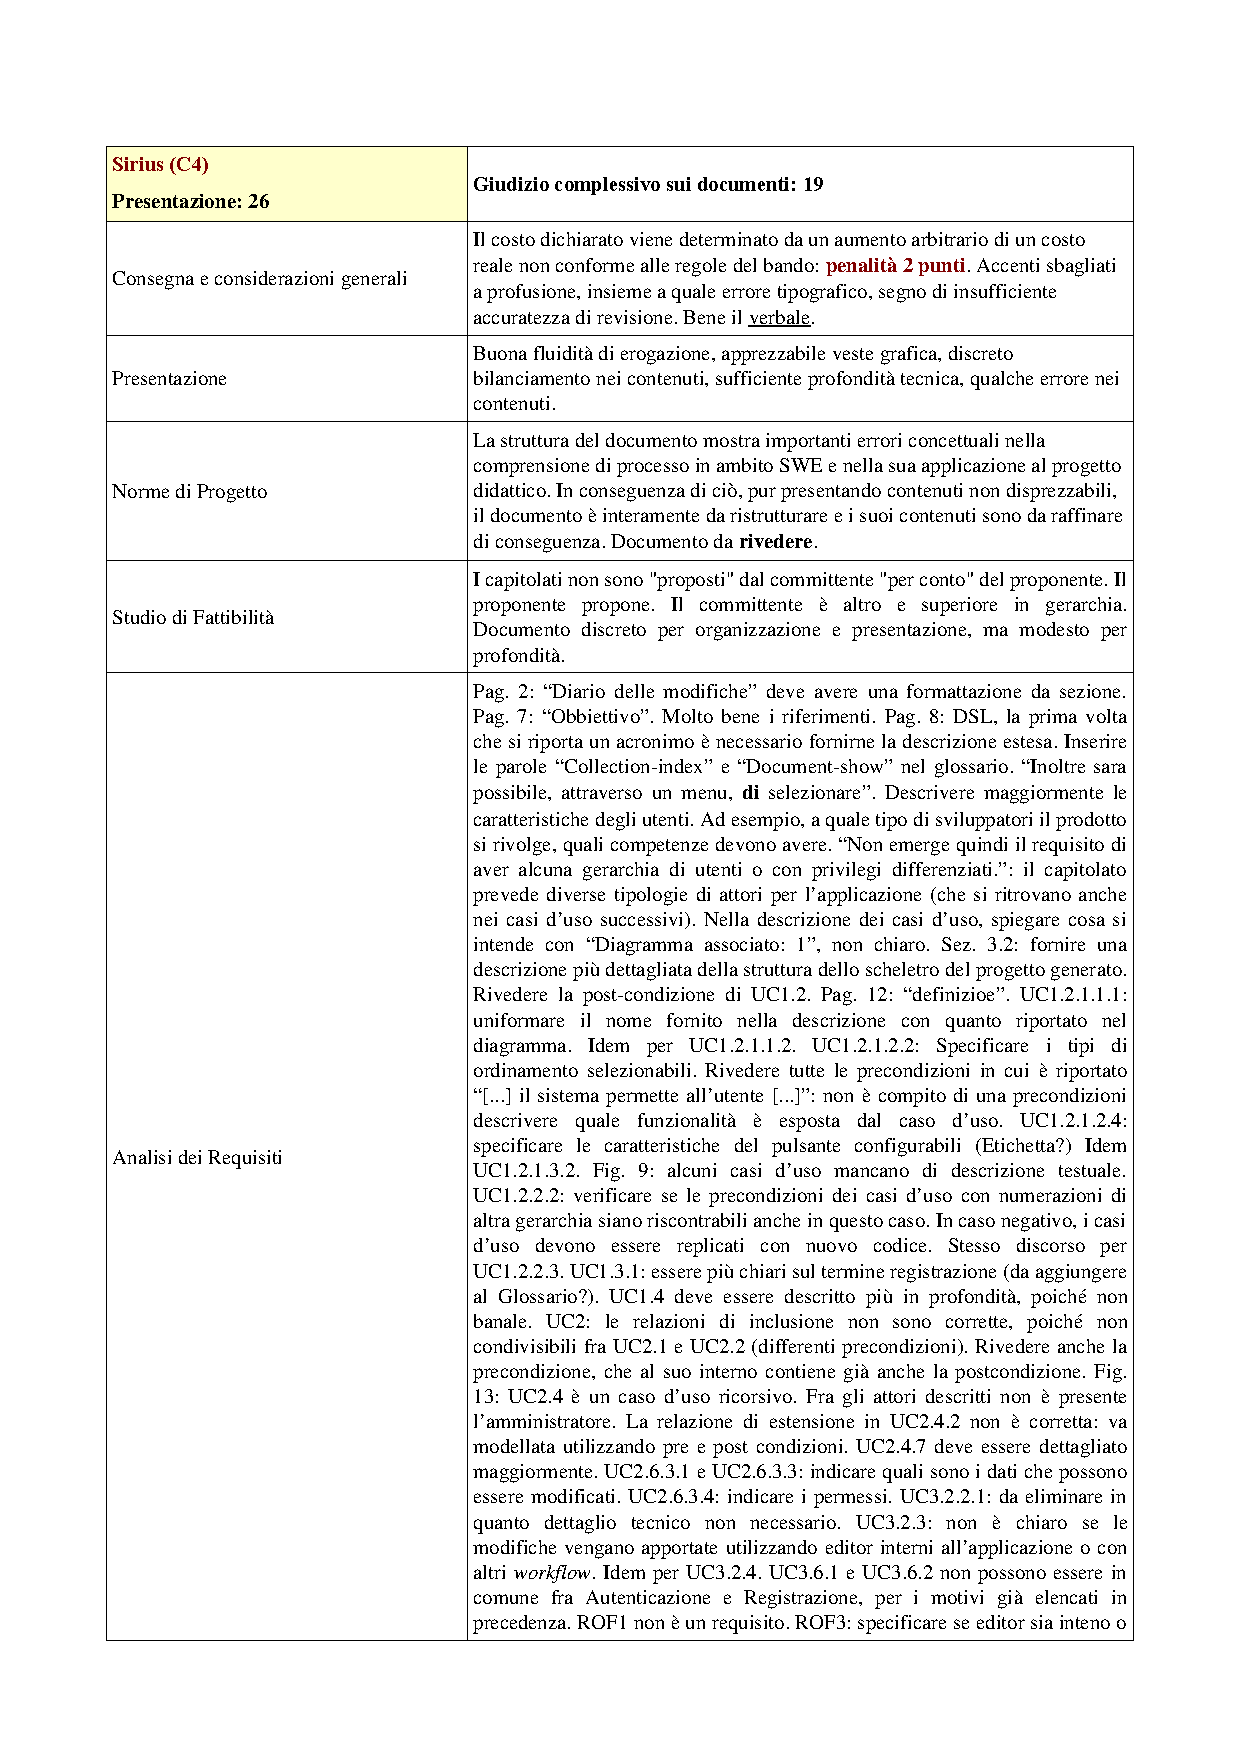
\includegraphics[scale=0.001]{img/Sirius.png}}
        \end{picture}}
	\rhead{\groupname}
	\chead{}
	\lfoot{\info}
	\cfoot{}
%	\rfoot{\thepage}
	\rfoot{\thepage\ / \pageref{LastPage}}
	\renewcommand{\headrulewidth}{0.3pt}
	\renewcommand{\footrulewidth}{0.3pt}
\linespread{1.2}	% valore interlinea


\fancypagestyle{romano}{
	\lhead{\setlength{\unitlength}{1mm}
        \begin{picture}(0,0)
                \put(5,0){
\includegraphics[scale=0.03]{../modello/img/sirius.png}}
        \end{picture}}
	\chead{}
	\rhead{\groupname}
	\lfoot{\info}
	\cfoot{}
	\rfoot{\thepage}
	\renewcommand{\headrulewidth}{0.3pt}
	\renewcommand{\footrulewidth}{0.3pt}
}



\hypersetup{
    colorlinks=true,linkcolor=[rgb]{0.11,0.55,0.83
    },          % colore link interni
    urlcolor=cyan           %colore link esterni
}
\definecolor{err}{rgb}{0.9,0.1,0.1}
\definecolor{rt}{rgb}{0.1,0.6,0.8}
\definecolor{grey}{rgb}{0.4,0.3,0.4}
\definecolor{mycolor}{rgb}{0.67,1,0.18}

\bibliographystyle{plain_ita}%bibliografia stile italiano

\pagenumbering{Roman}
\setlength\parindent{0pt} % sempre senza indentatura
% fine layout% layout

\makeatletter
\renewcommand*{\BreakableSlash}{%
  \leavevmode
  \prw@zbreak
  %
  \discretionary{-}{}{}%
  \prw@zbreak
}

\tolerance 1414
\hbadness 1414
\emergencystretch 1.5em
\hfuzz 0.3pt
\widowpenalty=10000
\vfuzz \hfuzz
\raggedbottom

\begin{document}

% Prima pagina di opgni documento
\begin{titlepage}
 \begin{center}
     
\includegraphics[width=11cm]{../modello/img/sirius}\\
     \vspace{1em}
     {\LARGE \textsc{Sirius}}\\
     \vspace{2em} \hrule \vspace{2em}
     {\Large \textsc{Sequenziatore}}\\
     \vspace{8em}
     {\LARGE \LARGE \LARGE \textbf{\doctitle}}\\
     \vspace{2em}
     {\LARGE \LARGE \LARGE \textbf{Versione \lastversion }}\\
     \vspace{4em}
 \end{center}


\vskip 1.8cm
\begin{center}
\textit{Ingegneria Del Software AA 2013-2014}
\end{center}

\end{titlepage}


%pagina del titolo
\thispagestyle{romano}
\noindent\begin{Large}\textbf{Informazioni documento}\end{Large}\\
\begin{center}
\begin{tabular}{ll}
\hline\\
Titolo documento: & Analisi dei requisiti\\
Data creazione: & 1 Febbraio 2014\\
Versione attuale: & \lastversion\\
Utilizzo: & Esterno\\
Nome file:& \AnalisiDeiRequisiti{}\\
Redazione: & Botter Marco\\
& Giachin Vanni\\
& Marcomin Gabriele\\
Verifica: & Seresin Davide\\
Approvazione: & Quaglio Davide\\
Distribuito da:& Sirius\\
Destinato a: & Prof. Vardanega Tullio\\
			 & Prof. Cardin Riccardo\\
			 & Zucchetti S.p.A.
\end{tabular}
\end{center}
\vskip 1.5cm
%\noindent {\begin{LARGE}\textbf{Sommario}\end{LARGE}}\\
\noindent\begin{Large}\textbf{Sommario}\end{Large}\\

\noindent Risultato dello studio di fattibilità della ditta Sirius per il capitolato C04 Seq\\
\newpage
\pagestyle{romano}
\noindent\begin{Large}\textbf{Diario delle modifiche}\end{Large}\\
\\
%Inserire in testa ogni nuova versione\\
\begin{small}
\begin{tabular}{|c|p{1.8cm}|p{2.8cm}|p{2.8cm}|p{3.5cm}|}
\hline
Versione & Data & Autore & Ruolo & Descrizione \\
\hline
\hline
1.0.0 & 2014-03-05 & 
\textit{Quaglio Davide} &
\textit{Responsabile} &  Approvazione del documento\\
\hline
0.1.0 & 2014-02-13 & 
\textit{Botter Marco} &
\textit{Verificatore} &  Verifica del documento\\
\hline
0.0.2 & 2014-02-11 & 
\textit{Seresin Davide} &
\textit{Analista} &  Aggiunte e modifiche\\
\hline
0.0.1 & 2014-02-09 & 
\textit{Santangelo Davide} &
\textit{Analista} &  Creato lo scheletro del documento\\
\hline
\end{tabular}\\
\end{small}


\newpage
\pagestyle{romano}

\tableofcontents %sommario
\pagestyle{romano}



\newpage
\pagestyle{plain}
%\listoftables
%\listoffigures
\pagenumbering{arabic}%numeri di pagina  arabi

% VIEW
\newcommand{\client}{com.si\fshyp{}ri\fshyp{}us.se\fshyp{}quen\fshyp{}zia\fshyp{}to\fshyp{}re.cli\fshyp{}ent}
\newcommand{\server}{com.si\fshyp{}ri\fshyp{}us.se\fshyp{}quen\fshyp{}zia\fshyp{}to\fshyp{}re.ser\fshyp{}ver}
\newcommand{\view}{com.si\fshyp{}ri\fshyp{}us.se\fshyp{}quen\fshyp{}zia\fshyp{}to\fshyp{}re.cli\fshyp{}ent.view}


\newcommand{\viewAdmin}{com.si\fshyp{}ri\fshyp{}us.se\fshyp{}quen\fshyp{}zia\fshyp{}to\fshyp{}re.cli\fshyp{}ent.view.pro\fshyp{}cess\fshyp{}ow\fshyp{}ner}

\newcommand{\viewUser}{com.si\fshyp{}ri\fshyp{}us.se\fshyp{}quen\fshyp{}zia\fshyp{}to\fshyp{}re.cli\fshyp{}ent.view.u\fshyp{}ser}

% PRESENTER

\newcommand{\logic}{com.si\fshyp{}ri\fshyp{}us.se\fshyp{}quen\fshyp{}zia\fshyp{}to\fshyp{}re.cli\fshyp{}ent.pre\fshyp{}sen\fshyp{}ter}

\newcommand{\logicAdmin}{com.si\fshyp{}ri\fshyp{}us.se\fshyp{}quen\fshyp{}zia\fshyp{}to\fshyp{}re.cli\fshyp{}ent.pre\fshyp{}sen\fshyp{}ter.pro\fshyp{}cess\fshyp{}ow\fshyp{}ner}

\newcommand{\logicUser}{com.si\fshyp{}ri\fshyp{}us.se\fshyp{}quen\fshyp{}zia\fshyp{}to\fshyp{}re.cli\fshyp{}ent.pre\fshyp{}sen\fshyp{}ter.u\fshyp{}ser}


% MODEL

\newcommand{\modelAdmin}{com.si\fshyp{}ri\fshyp{}us.se\fshyp{}quen\fshyp{}zia\fshyp{}to\fshyp{}re.cli\fshyp{}ent.mo\fshyp{}del.pro\fshyp{}cess\fshyp{}\_\fshyp{}ow\fshyp{}ner}

\newcommand{\modelUser}{com.si\fshyp{}ri\fshyp{}us.se\fshyp{}quen\fshyp{}zia\fshyp{}to\fshyp{}re.cli\fshyp{}ent.mo\fshyp{}del.u\fshyp{}ser}

\newcommand{\model}{com.si\fshyp{}ri\fshyp{}us.se\fshyp{}quen\fshyp{}zia\fshyp{}to\fshyp{}re.cli\fshyp{}ent.mo\fshyp{}del}

\newcommand{\collection}{com.si\fshyp{}ri\fshyp{}us.se\fshyp{}quen\fshyp{}zia\fshyp{}to\fshyp{}re.cli\fshyp{}ent.mo\fshyp{}del.col\fshyp{}lec\fshyp{}tion}

% SERVER
\newcommand{\sPresenter}{com.si\fshyp{}ri\fshyp{}us.se\fshyp{}quen\fshyp{}zia\fshyp{}to\fshyp{}re.ser\fshyp{}ver.pre\fshyp{}sen\fshyp{}ter}

\newcommand{\sCommunication}{com.si\fshyp{}ri\fshyp{}us.se\fshyp{}quen\fshyp{}zia\fshyp{}to\fshyp{}re.ser\fshyp{}ver.pre\fshyp{}sen\fshyp{}ter.com\fshyp{}mu\fshyp{}ni\fshyp{}ca\fshyp{}tion}

\newcommand{\sLogicUser}{com.si\fshyp{}ri\fshyp{}us.se\fshyp{}quen\fshyp{}zia\fshyp{}to\fshyp{}re.ser\fshyp{}ver.pre\fshyp{}sen\fshyp{}ter.u\fshyp{}ser}

\newcommand{\sLogicAdmin}{com.si\fshyp{}ri\fshyp{}us.se\fshyp{}quen\fshyp{}zia\fshyp{}to\fshyp{}re.ser\fshyp{}ver.pre\fshyp{}sen\fshyp{}ter.pro\fshyp{}cess\fshyp{}ow\fshyp{}ner}

\newcommand{\dao}{com.si\fshyp{}ri\fshyp{}us.se\fshyp{}quen\fshyp{}zia\fshyp{}to\fshyp{}re.ser\fshyp{}ver.mo\fshyp{}del.dao}

\newcommand{\daoUser}{com.si\fshyp{}ri\fshyp{}us.se\fshyp{}quen\fshyp{}zia\fshyp{}to\fshyp{}re.ser\fshyp{}ver.mo\fshyp{}del.dao\fshyp{}u\fshyp{}ser}

\newcommand{\daoAdmin}{com.si\fshyp{}ri\fshyp{}us.se\fshyp{}quen\fshyp{}zia\fshyp{}to\fshyp{}re.ser\fshyp{}ver.mo\fshyp{}del.dao\fshyp{}pro\fshyp{}cess\fshyp{}ow\fshyp{}ner}

\newcommand{\daoProcess}{com.si\fshyp{}ri\fshyp{}us.se\fshyp{}quen\fshyp{}zia\fshyp{}to\fshyp{}re.ser\fshyp{}ver.mo\fshyp{}del.dao\fshyp{}pro\fshyp{}cess}

\newcommand{\daoStep}{com.si\fshyp{}ri\fshyp{}us.se\fshyp{}quen\fshyp{}zia\fshyp{}to\fshyp{}re.ser\fshyp{}ver.mo\fshyp{}del.dao\fshyp{}step}

\newcommand{\smodel}{com.si\fshyp{}ri\fshyp{}us.se\fshyp{}quen\fshyp{}zia\fshyp{}to\fshyp{}re.ser\fshyp{}ver.mo\fshyp{}del}

\section{Introduzione}

\subsection{Scopo del documento}
Il documento definisce le norme, convenzioni e formalismi  che ciascun membro del gruppo \gruppo{} deve adottare durante l'intera produzione del software \progetto{}.
In particolare tali norme regolamentano i seguenti aspetti:

\begin{itemize}
\item Organizzazione tra i membri del gruppo;
\item Stili e convenzioni nella redazione dei documenti;
\item Metodi operativi e convenzioni nelle fasi di progetto;
\item Ambiente di lavoro.
\end{itemize}

\subsection{Glossario}
Al fine di facilitare la comprensione dei documenti, i termini tecnici, di dominio e gli acronimi, sono definiti in dettaglio nel documento GLOSSARIO.\\
Tali termini sono contrassegnati dal simbolo \ped{$\vert$G$\vert$} che li segue.
\section{Definizione dell' architettura}
\subsection{Metodo e formalismo di specifica}
L' architettura del sistema è la struttura del sistema, che comprende gli elementi \textit{software}, la visibilità esterna di questi elementi e la relazione tra loro.
Questo documento andrà ad esporre le componenti di alto livello del sistema che verranno poi approfondite nel periodo di Progettazione di dettaglio e codifica, per analizzare l' architettura del sistema il \progetto si seguirà l' approccio \textit{top-down}, quindi innanzitutto si analizzerà il sistema fornendone una descrizione generale per poi scomporre le varie parti andando sempre più in dettaglio analizzando le singole componenti.
Successivamente si analizzeranno i \textit{design pattern} adottati e come verranno implementati.
Per esporre al meglio l architettura del sistema e il suo funzionamento di alto livello si utilizzeranno diagrammi dei \textit{package}, delle classi, di attività e di sequenza seguendo quanto imposto dalle \NormeDiProgetto{}.
\subsection{Architettura generale}
Il sistema \progetto{} è composto innanzitutto da due parti principali, un lato \textit{Client} e un lato \textit{Server}, per la loro progettazione si è tenuto conto dei principi della \textbf{riusabilità} e del \textbf{basso accoppiamento}, quindi si cercherà di progettare le due parti distintamente e senza dipendenze mantenendo all' oscuro il funzionamento del \textbf{server} al \textbf{client} e viceversa.\\
Dopo un' attenta analisi si è deciso di adottare il \textit{design pattern} architetturale \textbf{MVP} per quanto riguarda il client, seguendo la variante \textit{Passive View}. Tale scelta è stata fatta per i seguenti motivi:
\begin{itemize}
%490.317 visualizzazioni
	\item ottenere una \textit{view} priva di \textit{application logic} che verrà delegata al \textit{presenter}, questo semplificherà i test, infatti la vista sarà un semplice \textit{mockup} e il \textit{presenter} può essere testato separatamente dalla vista;
	\item offre un' architettura solida e mantenibile attraverso il disaccoppiamento massimo tra viste e modelli.
\end{itemize}
Per quanto riguarda il server si è implementato il design pattern \textbf{\textit{Three Tier}}, permettendo di sviluppare i singoli livelli come moduli indipendenti. Utilizzando questo design pattern abbiamo ottenuto la seguente divisione:
\begin{itemize}
	\item \textbf{Data Tier: } In questo livello verranno conservate le informazioni e recuperate dal database MySql. Le informazioni recuperate verranno poi passate al \textit{Logic Tier} per essere processate. 
	\item \textbf{Logic Tier: } Qui risiede l' \textit{application logic}, vengono eseguiti i comandi, vengono prese decisioni logiche e vengono eseguite le operazioni. Tutte le classi di questo \textit{tier} sono le classi \textit{service}.
	\item \textbf{Presentatin Tier: } Le operazioni eseguite dal precedente livello vengono passate ai controller, i quali passano al client l' esito delle operazioni che dovrà trasformare questi risultati per fornirli all' utente in modo che possa comprenderli, questo sarà lo scopo di questo livello.
\end{itemize}
\subsubsection{Componente View}
Questa componente andrà a costituire la \textbf{GUI} del sistema e sarà divisa in due parti, lato amministratore e quello utente. Entrambe le parti non dovranno fare altro che offrire un' interfaccia agli utenti del sistema utilizzando HTML5, CSS e Javascript.
\subsubsection{Componente Presenter}
Il \textit{presenter} andrà a rappresentare la \textit{application logic} del sistema \textit{client}. Le funzionalità che andrà a ricoprire saranno:
\begin{itemize}
	\item gestire parte della comunicazione tra \textit{client} e \textit{server};
	\item acquisire i dati inseriti dagli utenti e fornirne una prima elaborazione;
	\item aggiornare le viste dell' utente e dell' amministratore;
	\item passare i dati che necessitano di elaborazione lato \textit{server} allo stesso;
	\item ricevere le risposte dal lato \textit{server} e fornire all' utente la vista aggiornata.
\end{itemize}
\subsubsection{Componente Model}
Questa componente andrà a rappresentare la \textit{business logic} del sistema, e sarà suddivisa tra \textit{client} in minima parte e \textit{server}.
I ruoli del componente lato \textit{client} saranno di mantenere traccia dell' utente autenticato e di salvare, qualora si decida di implementare questa funzionalità, i dati come per esempio coordinate gps e immagini quando il dispositivo non disporrà di connessione internet.
\subsubsection{Componente Service}
Questa componente risiede nel server, tali classi saranno adibite a svolgere varie operazioni che il \textit{client} non è in grado di eseguire, come controllo della \textit{login} o la creazione di un nuovo utente nel sistema. Una volta eseguite le operazioni passerà l' esito di tali elaborazioni alla componente \textit{Controller}.
\subsubsection{Componente Controller}
Questa componente è incaricata di ricevere le richieste dal \textit{client} e delegarne l' elaborazione alla componente \textit{service} e di ritornare l' esito dei calcoli al \textit{client}.
\begin{figure}[H] \centering 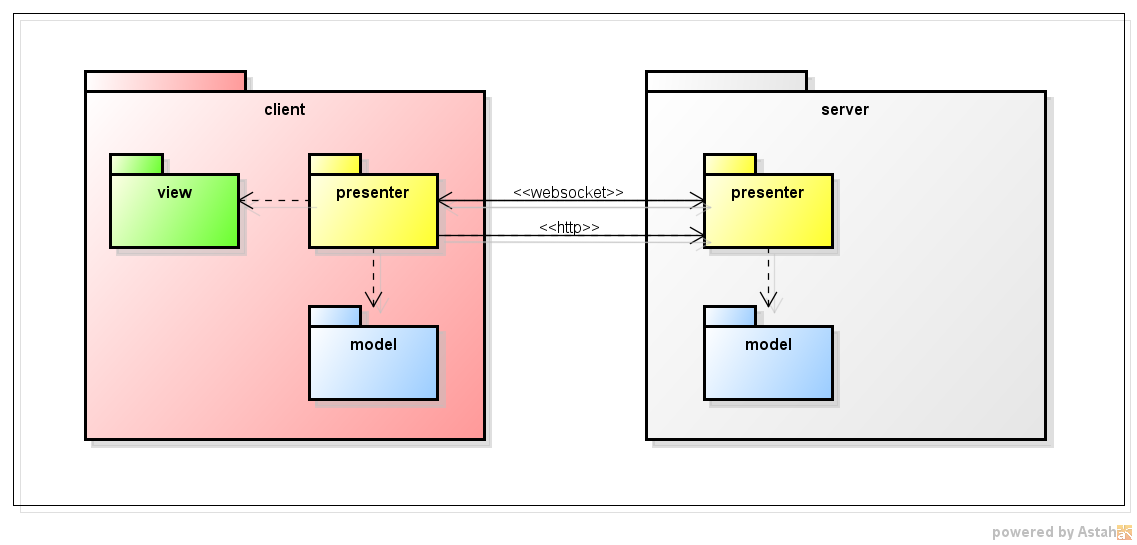
\includegraphics[width=%
\textwidth]
{./other/MVPIntroduzione.png} \caption{Diagramma UML architettura generale}
\end{figure}
\subsection{Diagrammi dei package}
Il seguente diagramma descrive le dipendenze intercorse fra i vari package\ped{G} del sistema Sequenziatore.
I diagrammi dei package |g| descrivono le dipendenze che intercorrono tra i vari
package\ped{G} che compongono il sistema.
Figura 3: Diagramma dei package del prodotto MyTalk.
Il sistema Sequenziatore è composto da due macro package\ped{G}:
\begin{enumerate}
	\item sequenziatore::client: le componenti di questo package\ped{G} realizzano la parte front-end\ped{G} del sistema Sequenziatore 
	\item sequenziatore::server: le componenti di questo package\ped{G} realizzano la parte back-end\ped{G} del sistema Sequenziatore 
\end{enumerate}
Il package\ped{G} sequenziatore.client è composto dai seguenti package\ped{G}:
\begin{itemize}
	\item sequenziatore::client::view;
	\item sequenziatore::client::presenter;
	\item sequenziatore::client::model.
\end{itemize}
Come è facilmente intuibile, la struttura del package\ped{G} sequenziatore.client si basa sulla struttura del design patter
architetturale Model View Presenter, scelto dal team Sirius per poter separare la logica di presentazione dei dati dalla logica di business.\\
I package\ped{G} che compongono il package\ped{G} sequenziatore::server sono:
\begin{itemize}
	\item sequenziatore::server::presenter;
	\item sequenziatore::server::model.
\end{itemize}
\subsubsection{Package sequenziatore::client::view}
Il package\ped{G} sequenziatore::client::view è composto da i seguenti package\ped{G}:
\begin{itemize}
	\item sequenziatore::client::view::process_owner: contiene le componenti template necessarie per la realizzazione dell’interfaccia grafica del process owner.
	\item sequenziatore::client::view::user: contiene le componenti template necessarie per la realizzazione dell’interfaccia grafica dell'user.
\end{itemize}
\subsubsection{Package sequenziatore::client::presenter}
Il package\ped{G} sequenziatore::client::presenter contiene tutte le componenti del Presenter della parte client\ped{G} del sistema Sequenziatore; ed è composto da i seguenti package\ped{G}:
\begin{itemize}
	\item sequenziatore::client::presenter::process_owner: contiene le componenti che costituiscono la componente Presenter
per il process owner, il package\ped{G} sequenziatore::client::presenter::process_owner è diviso ulteriormente nei sotto-package\ped{G}:
	\begin{itemize}
		\item sequenziatore::client::presenter::process_owner::views: contiene le classi necessarie per realizzare e gestire l'aggiornamento della parte grafica, usando i template presenti nel package\ped{g} sequenziatore::client::view::process_owner, e alla gestione degli eventi generati dall'interazione da parte del process owner con l'interfaccia grafica, gestendo inoltre la logica di business dell'applicazione;
	\end{itemize}
	\item sequenziatore::client::presenter::user: contiene le componenti che realizzano la componente Presenter per l'utente autenticato; i sotto-package\ped{G} di sequenziatore::client::presenter::user sono i seguenti:
	\begin{itemize}
		\item sequenziatore::client::presenter::user::views: contiene le classi necessarie per realizzare, mediante i template presenti nel package\ped{g} sequenziatore::client::view::user, l'interfaccia utente e gestirne l'interazione con l'utente autenticato, gestendo inoltre la logica di business dell'applicazione;
	\end{itemize}
\end{itemize}
\subsubsection{Package sequenziatore::client::model}
Il package\ped{G} sequenziatore::client::model contiene tutte le classi della componente Model. 
Il package\ped{G} sequenziatore::client::model contiene inoltre:
\begin{itemize}
	\item sequenziatore::client::model::collections contiene le varie collezioni di dati contenuti nel package model; il nome del package ricalca inoltre il nome del supertipo di tutte le collezioni di strutture date usate in un sistema sviluppato usando il framework\ped{G} Backbone.js\ped{G}
\end{itemize}

\section{Descrizione singoli componenti}
\subsection{Package sequenziatore.client.view}
\subsubsection{Package sequenziatore::client::iview::iuser}

\paragraph{IMainUser}
\begin{itemize}
\item \textbf{Nome:} \texttt{IMainUser};
\item \textbf{Package:} \texttt{\iViewUser{}};
\item \textbf{Descrizione:} Interfaccia che permette la gestione delle principali componenti dell'Interfaccia grafica dell'utente.
\end{itemize}

\paragraph{IUpdateView}
\begin{itemize}
\item \textbf{Nome:} \texttt{IUpdateView};
\item \textbf{Package:} \texttt{\iViewUser{}};
\item \textbf{Descrizione:} Interfaccia che permette di gestire l’aggiornameno dei \textit{widget\ped{G}} della componente \textit{view};
\end{itemize}

\paragraph{ILogin}
\begin{itemize}
\item \textbf{Nome:} \texttt{ILogin};
\item \textbf{Package:} \texttt{\iViewUser{}};
\item \textbf{Descrizione:} Interfaccia che permette di gestire l'interfaccia grafica relativa alle richieste di autenticazione e chiusura della sessione da parte dell'utente.
\end{itemize}

\paragraph{IRegister}
\begin{itemize}
\item \textbf{Nome:} \texttt{IRegister};
\item \textbf{Package:} \texttt{\iViewUser{}};
\item \textbf{Descrizione:} Interfaccia che permette di gestire l'interfaccia grafica relativa alle richieste di registrazione da parte dell'utente.
\end{itemize}

\paragraph{IViewData}
\begin{itemize}
\item \textbf{Nome:} \texttt{IViewData};
\item \textbf{Package:} \texttt{\iViewUser{}};
\item \textbf{Descrizione:} Interfaccia che permette la realizzazione dei \textit{widget} per la visualizzazione dei dati dell'utente.
\end{itemize}

\paragraph{IEditData}
\begin{itemize}
\item \textbf{Nome:} \texttt{IEditData};
\item \textbf{Package:} \texttt{\iViewUser{}};
\item \textbf{Descrizione:} Interfaccia che permette la realizzazione dei \textit{widget} per la modifica dei dati personali dell'utente.
\end{itemize}

\paragraph{IChangePassword}
\begin{itemize}
\item \textbf{Nome:} \texttt{IChangePassword};
\item \textbf{Package:} \texttt{\iViewUser{}};
\item \textbf{Descrizione:} Interfaccia che permette la realizzazione dei \textit{widget} per la modifica della \textit{password} dell'utente.
\end{itemize}

\paragraph{IOpenProcess}
\begin{itemize}
\item \textbf{Nome:} \texttt{IOpenProcess};
\item \textbf{Package:} \texttt{\iViewUser{}};
\item \textbf{Descrizione:} Interfaccia che permette di realizzare i \textit{widget} per consentire la ricerca e la selezione di processi.
\end{itemize}

\paragraph{IManagementSelectedProcess}
\begin{itemize}
\item \textbf{Nome:} \texttt{IManagementSelectedProcess};
\item \textbf{Package:} \texttt{\iViewUser{}};
\item \textbf{Descrizione:} Interfaccia che permette di realizzare i \textit{widget} per visualizzare lo stato corrente del processo selezionato e i vincoli per concludere il passo.
\end{itemize}

\paragraph{ISendData}
\begin{itemize}
\item \textbf{Nome:} \texttt{ISendData};
\item \textbf{Package:} \texttt{\iViewUser{}};
\item \textbf{Descrizione:} Interfaccia che permette di realizzare i \textit{widget} per inviare i dati richiesti per la conclusione del passo.
\end{itemize}

\paragraph{ISendText}
\begin{itemize}
\item \textbf{Nome:} \texttt{ISendData};
\item \textbf{Package:} \texttt{\iViewUser{}};
\item \textbf{Descrizione:} Interfaccia che permette di realizzare i \textit{widget} per inserire il testo da inviare per concludere il passo.
\end{itemize}

\paragraph{ISendNumb}
\begin{itemize}
\item \textbf{Nome:} \texttt{ISendNumb};
\item \textbf{Package:} \texttt{\iViewUser{}};
\item \textbf{Descrizione:} Interfaccia che permette di realizzare i \textit{widget} per inserire i dati numerici da inviare per concludere il passo.
\end{itemize}

\paragraph{ISendPosition}
\begin{itemize}
\item \textbf{Nome:} \texttt{ISendPosition};
\item \textbf{Package:} \texttt{\iViewUser{}};
\item \textbf{Descrizione:} Interfaccia che permette  di realizzare i \textit{widget} per inviare la posizione geografica per la conclusione di un passo. Inoltre consente di visualizzare eventuali messaggi d'errore nella rilevazione delle coordinate.
\end{itemize}

\paragraph{ISendImage}
\begin{itemize}
\item \textbf{Nome:} \texttt{ISendImage};
\item \textbf{Package:} \texttt{\iViewUser{}};
\item \textbf{Descrizione:} Interfaccia che permette di realizzare i \textit{widget} per inserire le immagini richieste per la conclusione del passo.
\end{itemize}

\paragraph{ISendPhoto}
\begin{itemize}
\item \textbf{Nome:} \texttt{ISendPhoto};
\item \textbf{Package:} \texttt{\iViewUser{}};
\item \textbf{Descrizione:} Interfaccia che permette di realizzare i \textit{widget} per consentire all'utente di scattare le fotografie richieste dal passo in esecuzione, e di inviarle.
\end{itemize}

\paragraph{IEndSelectedProcess}
\begin{itemize}
\item \textbf{Nome:} \texttt{IEndSelectedProcess};
\item \textbf{Package:} \texttt{\iViewUser{}};
\item \textbf{Descrizione:} Interfaccia che permette di realizzare i \textit{widget} per visualizzare l'esito del processo e consentire le operazioni di conclusione del processo.
\end{itemize}

\paragraph{IPrintProcess}
\begin{itemize}
\item \textbf{Nome:} \texttt{IPrintProcess};
\item \textbf{Package:} \texttt{\iViewUser{}};
\item \textbf{Descrizione:} Interfaccia che permette di realizzare i \textit{widget} per consentire il salvataggio dei \textit{report} di fine processo.
\end{itemize}

\paragraph{IPreviewProcess}
\begin{itemize}
\item \textbf{Nome:} \texttt{IPreviewProcess};
\item \textbf{Package:} \texttt{\iViewUser{}};
\item \textbf{Descrizione:} Interfaccia che permette di realizzare i \textit{widget} per consentire la visualizzazione dei \textit{report} di fine processo.
\end{itemize}
\subsubsection{Package sequenziatore::client::iview::iprocessowner}

\paragraph{IMainProcessOwner}
\begin{itemize}
\item \textbf{Nome:} \texttt{IMainProcessOwner};
\item \textbf{Package:} \texttt{\iViewAdmin{}};
\item \textbf{Descrizione:} Interfaccia che permette la gestione delle principali componenti dell'interfaccia grafica dell'utente \textit{process owner\ped{G}}.
\end{itemize}

\paragraph{IUpdateView}
\begin{itemize}
\item \textbf{Nome:} \texttt{IUpdateView};
\item \textbf{Package:} \texttt{\iViewAdmin{}};
\item \textbf{Descrizione:} Interfaccia che permette di gestire l'aggiornamento dei \textit{widget\ped{G}} della componente \textit{view}.
\end{itemize}

\paragraph{ILogin}
\begin{itemize}
\item \textbf{Nome:} \texttt{ILogin};
\item \textbf{Package:} \texttt{\iViewAdmin{}};
\item \textbf{Descrizione:} Interfaccia che permette di gestire l'interfaccia grafica relativa alle richieste di autenticazione e chiusura della sessione da parte dell'utente \textit{process owner\ped{G}}.
\end{itemize}

\paragraph{ISetProcess}
\begin{itemize}
\item \textbf{Nome:} \texttt{ISetProcess};
\item \textbf{Package:} \texttt{\iViewAdmin{}};
\item \textbf{Descrizione:} Interfaccia che permette di gestire l'interfaccia grafica che consente di creare nuovi processi.
\end{itemize}

\paragraph{IAddStep}
\begin{itemize}
\item \textbf{Nome:} \texttt{IAddStep};
\item \textbf{Package:} \texttt{\iViewAdmin{}};
\item \textbf{Descrizione:} Interfaccia che permette di gestire l'interfaccia grafica che consente di definire un nuovo passo del processo in creazione.
\end{itemize}

\paragraph{IPreviewProcess}
\begin{itemize}
\item \textbf{Nome:} \texttt{IPreviewProcess};
\item \textbf{Package:} \texttt{\iViewAdmin{}};
\item \textbf{Descrizione:} Interfaccia che permette realizzare i \textit{widget} che consentono di visualizzare l'anteprima del processo in creazione.
\end{itemize}

\paragraph{IOpenProcess}
\begin{itemize}
\item \textbf{Nome:} \texttt{IOpenProcess};
\item \textbf{Package:} \texttt{\iViewAdmin{}};
\item \textbf{Descrizione:} Interfaccia che permette di realizzare i \textit{widget} che consentono di aprire un processo tramite ricerca o selezione da una lista.
\end{itemize}

\paragraph{IManagmentSelectedProcess}
\begin{itemize}
\item \textbf{Nome:} \texttt{IManagmentSelectedProcess};
\item \textbf{Package:} \texttt{\iViewAdmin{}};
\item \textbf{Descrizione:} Interfaccia che permette di realizzare i \textit{widget} che consentono di gestire i processi selezionati.
\end{itemize}

\paragraph{ICheckStep}
\begin{itemize}
\item \textbf{Nome:} \texttt{ICheckStep};
\item \textbf{Package:} \texttt{\iViewAdmin{}};
\item \textbf{Descrizione:} Interfaccia che permette di realizzare i \textit{widget} che consentono di gestire il controllo dei passi che richiedono intervento umano.
\end{itemize}

\paragraph{IStatistics}
\begin{itemize}
\item \textbf{Nome:} \texttt{IStatistics};
\item \textbf{Package:} \texttt{\iViewAdmin{}};
\item \textbf{Descrizione:} Interfaccia che permette di realizzare i \textit{widget} che consentono di gestire l'accesso alle informazioni statistiche sui processi.
\end{itemize}

\paragraph{IUserReceivedData}
\begin{itemize}
\item \textbf{Nome:} \texttt{IUserReceivedData};
\item \textbf{Package:} \texttt{\iViewAdmin{}};
\item \textbf{Descrizione:} Classe che permette di realizzare i \textit{widget} che consentono di gestire l'accesso ai dati inviati al \textit{server\ped{G}} dagli utenti;
\end{itemize}

\paragraph{IInviteUser}
\begin{itemize}
\item \textbf{Nome:} \texttt{IInviteUser};
\item \textbf{Package:} \texttt{\iViewAdmin{}};
\item \textbf{Descrizione:} Interfaccia che permette di realizzare i \textit{widget} che consentono di gestire i permessi di iscrizione ad un processo da parte degli utenti.
\end{itemize}

\subsection{Package sequenziatore::client::view}
\subsubsection{Package sequenziatore.client.view.user}

\paragraph{IMainUser}
\begin{itemize}
\item \textbf{Nome:} \texttt{IMainUser};
\item \textbf{Descrizione:} Interfaccia che permette la gestione delle principali componenti dell'Interfaccia grafica dell'utente.
\end{itemize}

\paragraph{MainUser}
\begin{flushleft}
\begin{itemize}
\item \textbf{Nome:} \texttt{MainUser};
\item \textbf{Descrizione:} Classe che permette la gestione delle principali componenti dell'interfaccia grafica dell'utente;
\item \textbf{Relazioni con altri componenti:
\begin{sloppypar}
La classe implementa l'interfaccia \texttt{I\fshyp{}Main\fshyp{}U\fshyp{}ser}.
\end{sloppypar}
\end{itemize}
\end{flushleft}

\paragraph{ILogin}
\begin{itemize}
\item \textbf{Nome:} \texttt{ILogin};
\item \textbf{Descrizione:} Interfaccia che permette di gestire l'interfaccia grafica relativa alle richieste di autenticazione e chiusura della sessione da parte dell'utente.
\end{itemize}

\paragraph{Login}
\begin{flushleft}
\begin{itemize}
\item \textbf{Nome:} \texttt{Login};
\item \textbf{Descrizione:} Classe che permette di gestire dell'interfaccia grafica relativa alle richieste di autenticazione e chiusura della sessione da parte dell'utente;
\item \textbf{Relazioni con altri componenti:}
\begin{sloppypar}
La classe implementa l'interfaccia \texttt{I\fshyp{}Lo\fshyp{}gin}.
\end{sloppypar}
\end{itemize}
\end{flushleft}

\paragraph{IRegister}
\begin{itemize}
\item \textbf{Nome:} \texttt{IRegister};
\item \textbf{Package:} \texttt{\iViewUser{}};
\item \textbf{Descrizione:} Interfaccia che permette di gestire l'interfaccia grafica relativa alle richieste di registrazione da parte dell'utente.
\end{itemize}

\paragraph{Register}
\begin{flushleft}
\begin{itemize}
\item \textbf{Nome:} \texttt{Register};
\item \textbf{Descrizione:} Classe che permette di gestire dell'interfaccia grafica relativa alle richieste di registrazione da parte dell'utente;
\item \textbf{Relazioni con altri componenti:}
\begin{sloppypar}
La classe implementa l'interfaccia \texttt{I\fshyp{}Re\fshyp{}gis\fshyp{}ter}.
\end{sloppypar}
\end{itemize}
\end{flushleft}

\paragraph{IUserData}
\begin{itemize}
\item \textbf{Nome:} \texttt{IUserData};
\item \textbf{Descrizione:} Interfaccia che permette la realizzazione dei \textit{widget} per la visualizzazione dei dati dell'utente e la relativa modifica dei dati, dove possibile.
\end{itemize}

\paragraph{UserData}
\begin{flushleft}
\begin{itemize}
\item \textbf{Nome:} \texttt{UserData};
\item \textbf{Descrizione:} Classe che permette la realizzazione dei \textit{widget} che consentono visualizzazione e modifica dei dati dell'utente;
\item \textbf{Relazioni con altri componenti:}
\begin{sloppypar}
La classe implementa l'interfaccia \texttt{I\fshyp{}User\fshyp{}Da\fshyp{}ta}.
\end{sloppypar}
\end{itemize}
\end{flushleft}

\paragraph{IOpenProcess}
\begin{itemize}
\item \textbf{Nome:} \texttt{IOpenProcess};
\item \textbf{Descrizione:} Interfaccia che permette di realizzare i \textit{widget} per consentire la ricerca e la selezione di processi.
\end{itemize}

\paragraph{OpenProcess}
\begin{flushleft}
\begin{itemize}
\item \textbf{Nome:} \texttt{OpenProcess};
\item \textbf{Descrizione:} Classe che permette di realizzare i \textit{widget} per consentire l'apertura di un processo tramite ricerca o selezionandolo da una lista;
\item \textbf{Relazioni con altri componenti:}
\begin{sloppypar}
La classe implementa l'interfaccia \texttt{I\fshyp{}O\fshyp{}pen\fshyp{}Pro\fshyp{}cess}.
\end{sloppypar}
\end{itemize}
\end{flushleft}

\paragraph{IManagementProcess}
\begin{itemize}
\item \textbf{Nome:} \texttt{IManagementSelectedProcess};
\item \textbf{Descrizione:} Interfaccia che permette di realizzare i \textit{widget} per visualizzare lo stato corrente del processo selezionato e i vincoli per concludere il passo.
\end{itemize}

\paragraph{ManagementProcess}
\begin{flushleft}
\begin{itemize}
\item \textbf{Nome:} \texttt{ManagementProcess};
\item \textbf{Descrizione:} Classe che permette di realizzare i \textit{widget} per consentire la visualizzazione dello stato del processo selezionato e i vincoli per concludere il passo in corso;
\item \textbf{Relazioni con altri componenti:}
\begin{sloppypar}
La classe implementa l'interfaccia \texttt{I\fshyp{}Ma\fshyp{}na\fshyp{}ge\fshyp{}ment\fshyp{}Pro\fshyp{}cess}.
\end{sloppypar}
\end{itemize}
\end{flushleft}

\paragraph{ISendData}
\begin{itemize}
\item \textbf{Nome:} \texttt{ISendData};
\item \textbf{Descrizione:} Interfaccia che permette di realizzare i \textit{widget} per inviare i dati richiesti per la conclusione del passo.
\end{itemize}

\paragraph{SendData}
\begin{flushleft}
\begin{itemize}
\item \textbf{Nome:} \texttt{SendData};
\item \textbf{Descrizione:} Classe che permette di realizzare i \textit{widget} per consentire l'invio dei dati richiesti per la conclusione del passo in esecuzione;
\item \textbf{Relazioni con altri componenti:}
\begin{sloppypar}
La classe implementa l'interfaccia \texttt{\iViewUser{}::I\fshyp{}Send\fshyp{}Da\fshyp{}ta}.
\end{sloppypar}
\end{itemize}
\end{flushleft}

\paragraph{ISendText}
\begin{itemize}
\item \textbf{Nome:} \texttt{ISendData};
\item \textbf{Descrizione:} Interfaccia che permette di realizzare i \textit{widget} per inserire il testo da inviare per concludere il passo.
\end{itemize}

\paragraph{SendText}
\begin{flushleft}
\begin{itemize}
\item \textbf{Nome:} \texttt{SendData};
\item \textbf{Descrizione:} Classe che permette di realizzare i \textit{widget} che consentono di inserire il testo da inviare per concludere il passo in esecuzione;
\item \textbf{Relazioni con altri componenti:}
\begin{sloppypar}
La classe implementa l'interfaccia \texttt{\iViewUser{}::I\fshyp{}Send\fshyp{}Text}.
\end{sloppypar}
\end{itemize}
\end{flushleft}

\paragraph{ISendNumb}
\begin{itemize}
\item \textbf{Nome:} \texttt{ISendNumb};
\item \textbf{Descrizione:} Interfaccia che permette di realizzare i \textit{widget} per inserire i dati numerici da inviare per concludere il passo.
\end{itemize}

\paragraph{SendNumb}
\begin{flushleft}
\begin{itemize}
\item \textbf{Nome:} \texttt{SendNumb};
\item \textbf{Descrizione:} Classe che permette agli oggetti che la implementano di realizzare i \textit{widget} che consentono di inserire i dati numerici da inviare per concludere il passo in esecuzione;
\item \textbf{Relazioni con altri componenti:}
\begin{sloppypar}
La classe implementa l'interfaccia \texttt{I\fshyp{}Send\fshyp{}Numb}.
\end{sloppypar}
\end{itemize}
\end{flushleft}

\paragraph{ISendPosition}
\begin{itemize}
\item \textbf{Nome:} \texttt{ISendPosition};
\item \textbf{Descrizione:} Interfaccia che permette  di realizzare i \textit{widget} per inviare la posizione geografica per la conclusione di un passo. Inoltre consente di visualizzare eventuali messaggi d'errore nella rilevazione delle coordinate.
\end{itemize}

\paragraph{SendPosition}
\begin{flushleft}
\begin{itemize}
\item \textbf{Nome:} \texttt{SendPosition};
\item \textbf{Descrizione:} Classe che permette  di realizzare i \textit{widget} che consentono di inviare la posizione geografica richiesta per la conclusione del passo in esecuzione;
\item \textbf{Relazioni con altri componenti:}
\begin{sloppypar}
La classe implementa l'interfaccia \texttt{I\fshyp{}Send\fshyp{}Po\fshyp{}si\fshyp{}tion}.
\end{sloppypar}
\end{itemize}
\end{flushleft}

\paragraph{ISendImage}
\begin{itemize}
\item \textbf{Nome:} \texttt{ISendImage};
\item \textbf{Descrizione:} Interfaccia che permette di realizzare i \textit{widget} per inserire le immagini richieste per la conclusione del passo.
\end{itemize}

\paragraph{SendImage}
\begin{flushleft}
\begin{itemize}
\item \textbf{Nome:} \texttt{SendImage};
\item \textbf{Package:} \texttt{\viewUser{}};
\item \textbf{Descrizione:} Classe che permette di realizzare i \textit{widget} che consentono di inserire le immagini richieste per concludere i passo in esecuzione;
\item \textbf{Relazioni con altri componenti:}
\begin{sloppypar}
La classe implementa l'interfaccia \texttt{I\fshyp{}Send\fshyp{}Image}.
\end{sloppypar}
\end{itemize}
\end{flushleft}

\paragraph{IPrintProcess}
\begin{itemize}
\item \textbf{Nome:} \texttt{IPrintProcess};
\item \textbf{Descrizione:} Interfaccia che permette di realizzare i \textit{widget} per consentire il salvataggio dei \textit{report} di fine processo.
\end{itemize}

\paragraph{PrintProcess}
\begin{flushleft}
\begin{itemize}
\item \textbf{Nome:} \texttt{PrintProcess};
\item \textbf{Descrizione:} Classe che permette di realizzare i \textit{widget} che consentono il salvataggio dei \textit{report} sull'esecuzione del processo;
\item \textbf{Relazioni con altri componenti:}
\begin{sloppypar}
La classe implementa l'interfaccia \texttt{I\fshyp{}Print\fshyp{}Pro\fshyp{}cess}.
\end{sloppypar}
\end{itemize}
\end{flushleft}

\subsubsection{Package \viewAdmin{}}

\begin{figure}[H]
\centering
\includegraphics[trim=0cm 0.8cm 0cm 0cm,clip=true,scale=0.75]%
{./pack/POView.png} \caption{Diagramma \textit{view Process Owner} }
\end{figure}


\paragraph{IMainProcessOwner}
\begin{itemize}
\item \textbf{Nome:} \texttt{IMainProcessOwner};
\item \textbf{Package:} \texttt{\viewAdmin{}};
\item \textbf{Descrizione:} Interfaccia che permette la gestione delle principali componenti dell'interfaccia grafica dell'utente \textit{process owner\ped{G}}.
\end{itemize}

\paragraph{MainProcessOwner}
\begin{flushleft}
\begin{itemize}
\item \textbf{Nome:} \texttt{MainProcessOwner};
\item \textbf{Package:} \texttt{\viewAdmin{}};
\item \textbf{Descrizione:} Componente che permette la gestione delle principali componenti dell'interfaccia grafica dell'utente \textit{process owner\ped{G}};
\item \textbf{Relazioni con altri componenti:}
\begin{sloppypar}
Il componente implementa l'interfaccia \texttt{\viewAdmin{}.I\fshyp{}Main\fshyp{}Pro\fshyp{}cess\fshyp{}Ow\fshyp{}ner}.
\end{sloppypar}
\end{itemize}
\end{flushleft}

\paragraph{INewProcess}
\begin{itemize}
\item \textbf{Nome:} \texttt{INewProcess};
\item \textbf{Package:} \texttt{\viewAdmin{}};
\item \textbf{Descrizione:} Interfaccia che permette di gestire l'interfaccia grafica che consente di creare nuovi processi.
\end{itemize}

\paragraph{NewProcess}
\begin{flushleft}
\begin{itemize}
\item \textbf{Nome:} \texttt{NewProcess};
\item \textbf{Package:} \texttt{\viewAdmin{}};
\item \textbf{Descrizione:} Componente che permette di gestire l'interfaccia grafica che consente di creare nuovi processi;
\item \textbf{Relazioni con altri componenti:}
\begin{sloppypar}
Il componente implementa l'interfaccia \texttt{\viewAdmin{}.I\fshyp{}New\fshyp{}Pro\fshyp{}cess}.
\end{sloppypar}
\end{itemize}
\end{flushleft}

\paragraph{IAddStep}
\begin{itemize}
\item \textbf{Nome:} \texttt{IAddStep};
\item \textbf{Package:} \texttt{\viewAdmin{}};
\item \textbf{Descrizione:} Interfaccia che permette di gestire l'interfaccia grafica che consente di definire un nuovo passo del processo in creazione.
\end{itemize}

\paragraph{AddStep}
\begin{flushleft}
\begin{itemize}
\item \textbf{Nome:} \texttt{AddStep};
\item \textbf{Package:} \texttt{\viewAdmin{}};
\item \textbf{Descrizione:} Componente che permette di gestire l'interfaccia grafica che consente di definire un nuovo passo del processo in creazione;
\item \textbf{Relazioni con altri componenti:}
\begin{sloppypar}
Il componente implementa l'interfaccia \texttt{\viewAdmin{}.I\fshyp{}Add\fshyp{}Step}.
\end{sloppypar}
\end{itemize}
\end{flushleft}

\paragraph{IOpenProcess}
\begin{itemize}
\item \textbf{Nome:} \texttt{IOpenProcess};
\item \textbf{Package:} \texttt{\viewAdmin{}};
\item \textbf{Descrizione:} Interfaccia che permette di realizzare i \textit{widget} che consentono di aprire un processo tramite ricerca o selezione da una lista.
\end{itemize}

\paragraph{OpenProcess}
\begin{flushleft}
\begin{itemize}
\item \textbf{Nome:} \texttt{OpenProcess};
\item \textbf{Package:} \texttt{\viewAdmin{}};
\item \textbf{Descrizione:} Componente che permette di realizzare i\textit{widget} che consentono di aprire un processo tramite ricerca o selezionandolo da una lista;
\item \textbf{Relazioni con altri componenti:}
\begin{sloppypar}
Il componente implementa l'interfaccia \texttt{\viewAdmin{}.I\fshyp{}O\fshyp{}pen\fshyp{}Pro\fshyp{}cess}.
\end{sloppypar}
\end{itemize}
\end{flushleft}

\paragraph{IManageProcess}
\begin{itemize}
\item \textbf{Nome:} \texttt{IManageProcess};
\item \textbf{Package:} \texttt{\viewAdmin{}};
\item \textbf{Descrizione:} Interfaccia che permette di realizzare i\textit{widget} che consentono di gestire l'accesso ai dati inviati al\textit{server\ped{G}} dagli utenti;
\end{itemize}

\paragraph{ManageProcess}
\begin{flushleft}
\begin{itemize}
\item \textbf{Nome:} \texttt{ManageProcess};
\item \textbf{Package:} \texttt{\viewAdmin{}};
\item \textbf{Descrizione:} Componente che permette di realizzare i\textit{widget} che consentono di gestire l'accesso ai dati inviati al\textit{server\ped{G}} dagli utenti;
\item \textbf{Relazioni con altri componenti:}
\begin{sloppypar}
Il componente implementa l'interfaccia \texttt{\viewAdmin{}.I\fshyp{}Ma\fshyp{}na\fshyp{}ge\fshyp{}Pro\fshyp{}cess}.
\end{sloppypar}
\end{itemize}
\end{flushleft}

\paragraph{ICheckStep}
\begin{itemize}
\item \textbf{Nome:} \texttt{ICheckStep};
\item \textbf{Package:} \texttt{\viewAdmin{}};
\item \textbf{Descrizione:} Interfaccia che permette di realizzare i \textit{widget} che consentono di gestire il controllo dei passi che richiedono intervento umano.
\end{itemize}

\paragraph{CheckStep}
\begin{flushleft}
\begin{itemize}
\item \textbf{Nome:} \texttt{CheckStep};
\item \textbf{Package:} \texttt{\viewAdmin{}};
\item \textbf{Descrizione:} Componente che permette di realizzare i\textit{widget} che consentono di gestire l'approvazione dei passi che richiedono intervento umano;
\item \textbf{Relazioni con altri componenti:}
\begin{sloppypar}
Il componente implementa l'interfaccia \texttt{\viewAdmin{}.I\fshyp{}Check\fshyp{}Step}.
\end{sloppypar}
\end{itemize}
\end{flushleft}
\subsection{Package sequenziatore::client::ipresenter}
\subsubsection{Package sequenziatore::client::ipresenter::iuser::ilogic}
\begin{figure}[H] \centering 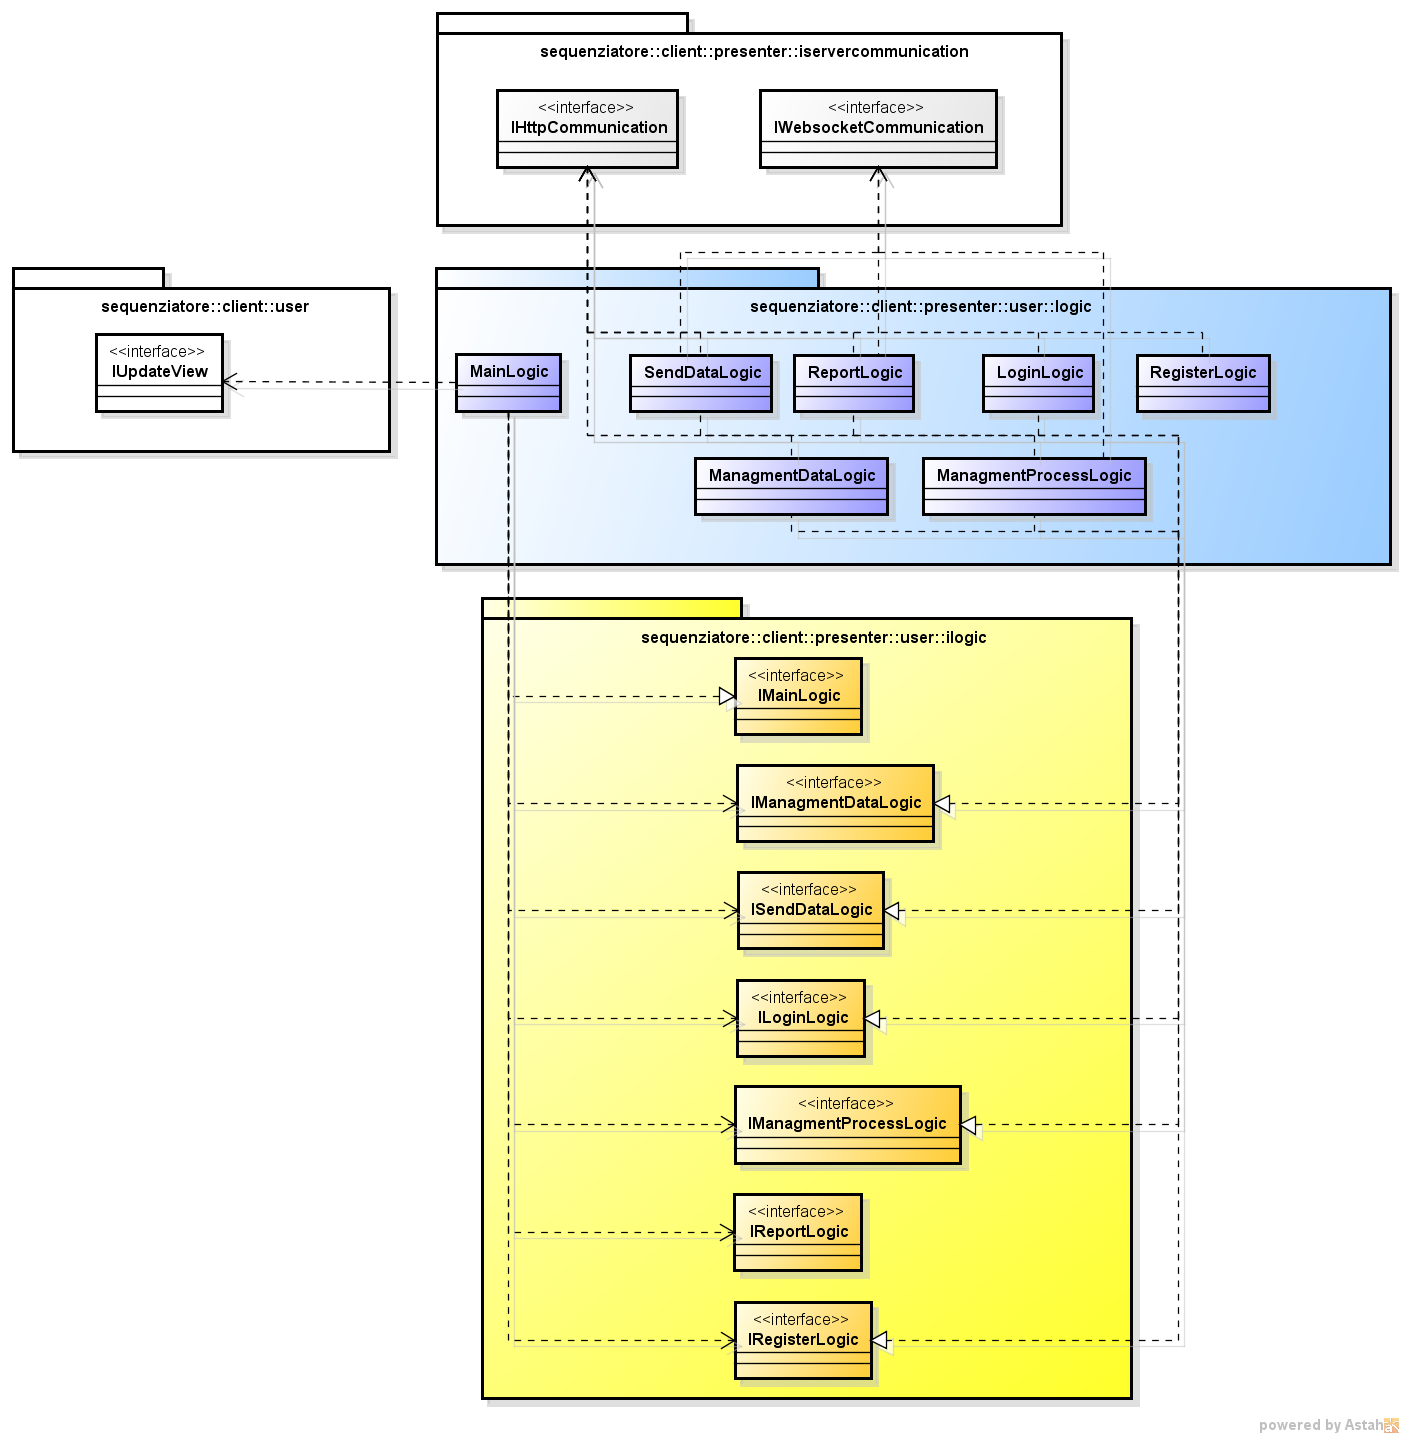
\includegraphics[width=%
\textwidth]
{./pack/presenter_user.png} \caption{Diagramma presenter user}
\end{figure}
\paragraph{IMainLogic}
\begin{itemize}
\item \textbf{Nome:} \texttt{IMainLogic};
\item \textbf{Package:} \texttt{\iLogicUser{}};
\item \textbf{Descrizione:} Interfaccia che permette di gestire gli eventi generati dalla componente \textit{View}.
\end{itemize}

\paragraph{ILoginLogic}
\begin{itemize}
\item \textbf{Nome:} \texttt{ILoginLogic};
\item \textbf{Package:} \texttt{\iLogicUser{}};
\item \textbf{Descrizione:} Interfaccia che ha il compito di gestire le richieste di autenticazione e chiusura della sessione da parte dell'utente.
\end{itemize}

\paragraph{IRegisterLogic}
\begin{itemize}
\item \textbf{Nome:} \texttt{IRegisterLogic};
\item \textbf{Package:} \texttt{\iLogicUser{}};
\item \textbf{Descrizione:} Interfaccia che ha il compito di gestire le richieste di registrazione da parte dell'utente.
\end{itemize}

\paragraph{IManagmentDataLogic}
\begin{itemize}
\item \textbf{Nome:} \texttt{IManagmentDataLogic};
\item \textbf{Package:} \texttt{\iLogicUser{}};
\item \textbf{Descrizione:} Interfaccia che ha il compito di gestire la visualizzazione e la modifica dei dati dell'utente.
\end{itemize}

\paragraph{IManagmentProcessLogic}
\begin{itemize}
\item \textbf{Nome:} \texttt{IManagmentProcessLogic};
\item \textbf{Package:} \texttt{\iLogicUser{}};
\item \textbf{Descrizione:} Interfaccia che ha il compito di gestire e accedere alle informazioni relative allo stato dei processi.
\end{itemize}

\paragraph{ISendDataLogic}
\begin{itemize}
\item \textbf{Nome:} \texttt{ISendDataLogic};
\item \textbf{Package:} \texttt{\iLogicUser{}};
\item \textbf{Descrizione:} Interfaccia che ha il compito di gestire l'inserimento e l'invio di dati da parte degli utenti.
\end{itemize}

\paragraph{IReportLogic}
\begin{itemize}
\item \textbf{Nome:} \texttt{IReportLogic};
\item \textbf{Package:} \texttt{\iLogicUser{}};
\item \textbf{Descrizione:} Interfaccia che ha il compito di gestire la creazione di report sull'andamento dei processi in esecuzione.
\end{itemize}
\subsubsection{Package sequenziatore::client::ipresenter::iprocessowner::ilogic}
\paragraph{IIMainLogic}
\begin{itemize}
\item \textbf{Nome:} \texttt{IMainLogic};
\item \textbf{Package:} \texttt{\iLogicAdmin{}};
\item \textbf{Descrizione:} Interfaccia che permette di gestire gli eventi generati dalla componente \textit{View};
\end{itemize}

\paragraph{ILoginLogic}
\begin{itemize}
\item \textbf{Nome:} \texttt{ILoginLogic};
\item \textbf{Package:} \texttt{\iLogicAdmin{}};
\item \textbf{Descrizione:} Interfaccia che ha il compito di gestire le richieste di autenticazione e chiusura della sessione da parte dell'utente \textit{process owner}.
\end{itemize}

\paragraph{INewProcessLogic}
\begin{itemize}
\item \textbf{Nome:} \texttt{INewProcessLogic};
\item \textbf{Package:} \texttt{\iLogicAdmin{}};
\item \textbf{Descrizione:} Interfaccia che ha il compito di gestire la logica della definizione di un nuovo processo.
\end{itemize}


\paragraph{IAddStepLogic}
\begin{itemize}
\item \textbf{Nome:} \texttt{IAddStepLogic};
\item \textbf{Package:} \texttt{\iLogicAdmin{}};
\item \textbf{Descrizione:} Interfaccia che ha il compito di definire la logica di gestione dei passi di un processo.
\end{itemize}


\paragraph{IManagmentProcessLogic}

\begin{itemize}
\item \textbf{Nome:} \texttt{IManagmentProcessLogic};
\item \textbf{Package:} \texttt{\iLogicAdmin{}};
\item \textbf{Descrizione:} Interfaccia che ha il compito di gestire e accedere alle informazioni relative allo stato dei processi.
\end{itemize}


\paragraph{ICheckStepLogic}
\begin{itemize}
\item \textbf{Nome:} \texttt{ICheckStepLogic};
\item \textbf{Package:} \texttt{\iLogicAdmin{}};
\item \textbf{Descrizione:} Interfaccia che ha il compito di definire la logica del controllo di un passo che richiede intervento umano per essere approvato.
\end{itemize}


\paragraph{IStatisticLogic}
\begin{itemize}
\item \textbf{Nome:} \texttt{IStatisticLogic};
\item \textbf{Package:} \texttt{\iLogicAdmin{}};
\item \textbf{Descrizione:} Interfaccia che ha il compito di gestire l'accesso alle informazioni statistiche sui processi.
\end{itemize}


\paragraph{IUserDataLogic}
\begin{itemize}
\item \textbf{Nome:} \texttt{IUserDataLogic};
\item \textbf{Package:} \texttt{\iLogicAdmin{}};
\item \textbf{Descrizione:} Interfaccia che ha il compito gestire l'accesso alle informazioni sui passi superati dagli utenti.
\end{itemize}


\paragraph{IInviteUserLogic}
\begin{itemize}
\item \textbf{Nome:} \texttt{IInviteUserLogic};
\item \textbf{Package:} \texttt{\iLogicAdmin{}};
\item \textbf{Descrizione:} Interfaccia che ha il compito di gestire i permessi di iscrizione ad un processo degli utenti.
\end{itemize}


\subsubsection{sequenziatore::client::ipresenter::iservercommunication}
\begin{figure}[H] \centering 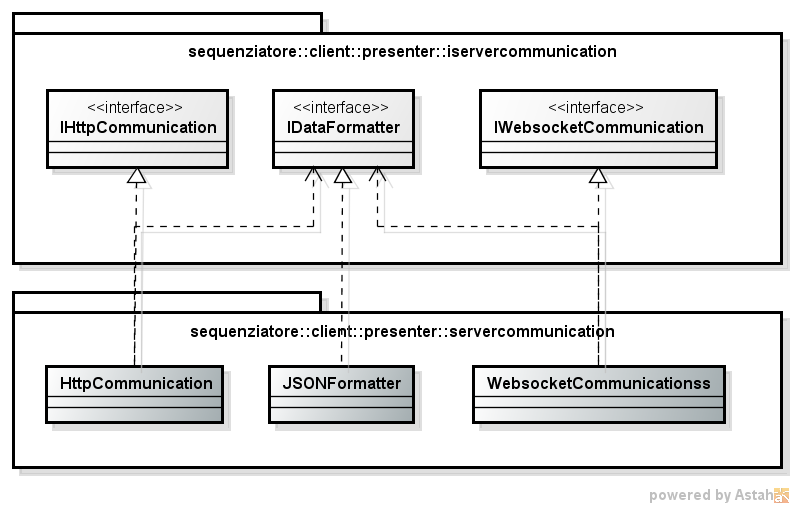
\includegraphics[width=%
\textwidth]
{./pack/servercommunication.png} \caption{Diagramma comunicazione con server}
\end{figure}
\paragraph{IHttpCommunication}
\begin{itemize}
\item \textbf{Nome:} \texttt{IHttpCommunication};
\item \textbf{Package:} \texttt{\serverCommunication{}};
\item \textbf{Descrizione:} Interfaccia che permette di gestire l'invio e ricezione di dati al \textit{server\ped{G}} tramite protocollo HTTP\ped{G}.
\end{itemize}

\paragraph{IWebsocketCommunication}
\begin{itemize}
\item \textbf{Nome:} \texttt{IWebsocketCommunication};
\item \textbf{Package:} \texttt{\serverCommunication{}};
\item \textbf{Descrizione:} Interfaccia che permette di gestire l'invio e ricezione di dati dal \textit{server\ped{G}} tramite \textit{websocket\ped{G}}.
\end{itemize}

\paragraph{IDataFormatter}
\begin{itemize}
\item \textbf{Nome:} \texttt{IDataFormatter};
\item \textbf{Package:} \texttt{\serverCommunication{}};
\item \textbf{Descrizione:} Interfaccia che permette di gestire la formattazione dei dati da inviare e ricevuti dal \textit{server\ped{G}}.
\end{itemize}

\subsection{Package sequenziatore::client::presenter}
\subsubsection{Package sequenziatore::client::presenter::user::logic}

\paragraph{MainLogic}
\begin{flushleft}
\begin{itemize}
\item \textbf{Nome:} \texttt{MainLogic};
\item \textbf{Package:} \texttt{\logicUser{}};
\item \textbf{Descrizione:} Classe che permette di gestire gli eventi generati dalla componente \textit{View};
\item \textbf{Relazioni con altri componenti:}
\begin{sloppypar}
La classe implementa l'interfaccia \texttt{\iLogicUser{}::I\fshyp{}Main\fshyp{}Lo\fshyp{}gic} e delega la gestione della logica di dettaglio alle seguenti classi:
\end{sloppypar}
\begin{itemize}
\item \texttt{\logicUser{}::Lo\fshyp{}gin\fshyp{}Lo\fshyp{}gic};
\item \texttt{\logicUser{}::Re\fshyp{}gis\fshyp{}ter\fshyp{}Lo\fshyp{}gic};
\item \texttt{\logicUser{}::Ma\fshyp{}nag\fshyp{}ment\fshyp{}Da\fshyp{}ta\fshyp{}Lo\fshyp{}gic};
\item \texttt{\logicUser{}::Ma\fshyp{}nag\fshyp{}ment\fshyp{}Pro\fshyp{}cess\fshyp{}Lo\fshyp{}gic};
\item \texttt{\logicUser{}::Send\fshyp{}Da\fshyp{}ta\fshyp{}Lo\fshyp{}gic};
\item \texttt{\logicUser{}::Re\fshyp{}port\fshyp{}Lo\fshyp{}gic};
\end{itemize}
\end{itemize}
\end{flushleft}

\paragraph{LoginLogic}
\begin{flushleft}
\begin{itemize}
\item \textbf{Nome:} \texttt{LoginLogic};
\item \textbf{Package:} \texttt{\logicUser{}};
\item \textbf{Descrizione:} Classe che ha il compito di gestire le richieste di autenticazione e chiusura della sessione da parte dell'utente;
\item \textbf{Relazioni con altri componenti:}
\begin{sloppypar}
La classe implementa l'interfaccia \texttt{\iLogicUser{}::I\fshyp{}Log\fshyp{}in\fshyp{}Lo\fshyp{}gic}, e utilizza metodi delle classi \texttt{\serverCommunication{}::Http\fshyp{}Com\fshyp{}mu\fshyp{}ni\fshyp{}ca\fshyp{}tion} e \texttt{\viewUser{}::Up\fshyp{}da\fshyp{}te\fshyp{}View}.
\end{sloppypar}
\end{itemize}
\end{flushleft}

\paragraph{RegisterLogic}
\begin{flushleft}
\begin{itemize}
\item \textbf{Nome:} \texttt{RegisterLogic};
\item \textbf{Package:} \texttt{\logicUser{}};
\item \textbf{Descrizione:} Classe che ha il compito di gestire le richieste di registrazione da parte dell'utente;
\item \textbf{Relazioni con altri componenti:}
\begin{sloppypar}
La classe implementa l'interfaccia \texttt{\iLogicUser{}::I\fshyp{}Re\fshyp{}gis\fshyp{}ter\fshyp{}Lo\fshyp{}gic}, e utilizza metodi delle classi \texttt{\serverCommunication{}::Http\fshyp{}Com\fshyp{}mu\fshyp{}ni\fshyp{}ca\fshyp{}tion} e \texttt{\viewUser{}::Up\fshyp{}da\fshyp{}te\fshyp{}View}.
\end{sloppypar}
\end{itemize}
\end{flushleft}

\paragraph{ManagmentDataLogic}
\begin{flushleft}
\begin{itemize}
\item \textbf{Nome:} \texttt{ManagmentDataLogic};
\item \textbf{Package:} \texttt{\logicUser{}};
\item \textbf{Descrizione:} Classe che ha il compito di gestire la visualizzazione e la modifica dei dati dell'utente;
\item \textbf{Relazioni con altri componenti:}
\begin{sloppypar}
La classe implementa l'interfaccia \texttt{\iLogicUser{}::I\fshyp{}Ma\fshyp{}na\fshyp{}gment\fshyp{}Da\fshyp{}ta\fshyp{}Lo\fshyp{}gic}, e utilizza metodi delle classi \texttt{\serverCommunication{}::Http\fshyp{}Com\fshyp{}mu\fshyp{}ni\fshyp{}ca\fshyp{}tion} e \texttt{\viewUser{}::Up\fshyp{}da\fshyp{}te\fshyp{}View}.
\end{sloppypar}
\end{itemize}
\end{flushleft}

\paragraph{ManagmentProcessLogic}
\begin{flushleft}
\begin{itemize}
\item \textbf{Nome:} \texttt{ManagmentProcessLogic};
\item \textbf{Package:} \texttt{\logicUser{}};
\item \textbf{Descrizione:} Classe che ha il compito di gestire e accedere alle informazioni relative allo stato dei processi. Le operazioni di gestione dello stato comprendono l'eliminazione dei processi terminati;
\item \textbf{Relazioni con altri componenti:}
\begin{sloppypar}
La classe implementa l'interfaccia \texttt{\iLogicUser{}::I\fshyp{}Ma\fshyp{}na\fshyp{}gment\fshyp{}Pro\fshyp{}cess\fshyp{}Lo\fshyp{}gic}, e utilizza metodi delle classi 
\texttt{\serverCommunication{}::Http\fshyp{}Com\fshyp{}mu\fshyp{}ni\fshyp{}ca\fshyp{}tion}, 
\texttt{\serverCommunication{}::Web\fshyp{}so\fshyp{}cket\fshyp{}Com\fshyp{}mu\fshyp{}ni\fshyp{}ca\fshyp{}tion}, \texttt{\modelUser{}::U\fshyp{}ser\fshyp{}Da\fshyp{}ta} e 
\texttt{\viewUser{}::Up\fshyp{}da\fshyp{}te\fshyp{}View}.
\end{sloppypar}
\end{itemize}
\end{flushleft}

\paragraph{SendDataLogic}
\begin{flushleft}
\begin{itemize}
\item \textbf{Nome:} \texttt{SendDataLogic};
\item \textbf{Package:} \texttt{\logicUser{}};
\item \textbf{Descrizione:} Classe che ha il compito di gestire l'inserimento e l'invio di dati da parte degli utenti;
\item \textbf{Relazioni con altri componenti:}
\begin{sloppypar}
La classe implementa l'interfaccia \texttt{\iLogicUser{}::I\fshyp{}Send\fshyp{}Da\fshyp{}ta\fshyp{}Lo\fshyp{}gic}, e utilizza metodi delle classi \texttt{\serverCommunication{}::Http\fshyp{}Com\fshyp{}mu\fshyp{}ni\fshyp{}ca\fshyp{}tion}, \texttt{\serverCommunication{}::Web\fshyp{}so\fshyp{}cket\fshyp{}Com\fshyp{}mu\fshyp{}ni\fshyp{}ca\fshyp{}tion}, \texttt{\model{}::U\fshyp{}ser\fshyp{}Da\fshyp{}ta} e \texttt{\viewUser{}::Up\fshyp{}da\fshyp{}te\fshyp{}View}.
\end{sloppypar}
\end{itemize}
\end{flushleft}

\paragraph{ReportLogic}
\begin{flushleft}
\begin{itemize}
\item \textbf{Nome:} \texttt{ReportLogic};
\item \textbf{Package:} \texttt{\logicUser{}};
\item \textbf{Descrizione:} Classe che ha il compito di gestire la creazione di report sull'andamento dei processi in esecuzione;
\item \textbf{Relazioni con altri componenti:}
\begin{sloppypar}
La classe implementa l'interfaccia \texttt{\iLogicUser{}::I\fshyp{}Ma\fshyp{}na\fshyp{}gment\fshyp{}Lo\fshyp{}gic}, e utilizza metodi delle classi \texttt{\serverCommunication{}::HttpCommunication}, \texttt{\serverCommunication{}::Web\fshyp{}so\fshyp{}cket\fshyp{}Com\fshyp{}mu\fshyp{}ni\fshyp{}ca\fshyp{}tion}, \texttt{\modelUser{}::U\fshyp{}ser\fshyp{}Da\fshyp{}ta} \texttt{\viewUser{}::Up\fshyp{}da\fshyp{}te\fshyp{}View}.
\end{sloppypar}
\end{itemize}
\end{flushleft}
\subsubsection{sequenziatore::client::presenter::processowner::logic}
\paragraph{MainLogic}
\begin{flushleft}
\begin{itemize}
\item \textbf{Nome:} \texttt{MainLogic};
\item \textbf{Package:} \texttt{\logicAdmin{}};
\item \textbf{Descrizione:} Classe che permette di gestire gli eventi generati dalla componente \textit{View};
\item \textbf{Relazioni con altri componenti:}
\begin{sloppypar}
La classe implementa l'interfaccia \texttt{\iLogicAdmin{}.I\fshyp{}Main\fshyp{}Lo\fshyp{}gic} e delega la gestione della logica di dettaglio alle seguenti classi:
\end{sloppypar}
\begin{itemize}
\item \texttt{\logicAdmin{}::Lo\fshyp{}gin\fshyp{}Lo\fshyp{}gic};
\item \texttt{\logicAdmin{}::New\fshyp{}Pro\fshyp{}cess\fshyp{}Lo\fshyp{}gic};
\item \texttt{\logicAdmin{}::Add\fshyp{}Step\fshyp{}Lo\fshyp{}gic};
\item \texttt{\logicAdmin{}::Ma\fshyp{}nag\fshyp{}ment\fshyp{}Pro\fshyp{}cess\fshyp{}Lo\fshyp{}gic};
\item \texttt{\logicAdmin{}::Check\fshyp{}Step\fshyp{}Lo\fshyp{}gic};
\item \texttt{\logicAdmin{}::Sta\fshyp{}tis\fshyp{}tics\fshyp{}Lo\fshyp{}gic};
\item \texttt{\logicAdmin{}::U\fshyp{}ser\fshyp{}Da\fshyp{}ta\fshyp{}Lo\fshyp{}gic};
\item \texttt{\logicAdmin{}::In\fshyp{}vi\fshyp{}te\fshyp{}U\fshyp{}ser\fshyp{}Lo\fshyp{}gic}.
\end{itemize}
\end{itemize}
\end{flushleft}

\paragraph{UpdateView}
\begin{flushleft}
\begin{itemize}
\item \textbf{Nome:} \texttt{LoginLogic};
\item \textbf{Package:} \texttt{\logicAdmin{}};
\item \textbf{Descrizione:} Classe che ha il compito di gestire l'aggiornameno dei \textit{widget\ped{G}} della componente \textit{View};
\item \textbf{Relazioni con altri componenti:}
\begin{sloppypar}
La classe implementa l'interfaccia \texttt{\iLogicAdmin{}::I\fshyp{}Up\fshyp{}date\fshyp{}View} e comunica con la \textit{View} utilizzando metodi della classe \texttt{\viewAdmin{}::Up\fshyp{}da\fshyp{}te\fshyp{}View}.
\end{sloppypar}
\end{itemize}
\end{flushleft}

\paragraph{LoginLogic}
\begin{flushleft}
\begin{itemize}
\item \textbf{Nome:} \texttt{LoginLogic};
\item \textbf{Package:} \texttt{\logicAdmin{}};
\item \textbf{Descrizione:} Classe che ha il compito di gestire le richieste di autenticazione e chiusura della sessione da parte dell'utente \textit{process owner};
\item \textbf{Relazioni con altri componenti:}
\begin{sloppypar}
La classe implementa l'interfaccia \texttt{\iLogicAdmin{}::I\fshyp{}Log\fshyp{}in\fshyp{}Lo\fshyp{}gic}, e utilizza metodi delle classi \texttt{\serverCommunication{}::Http\fshyp{}Com\fshyp{}mu\fshyp{}ni\fshyp{}ca\fshyp{}tion} e \texttt{\logicAdmin{}::Up\fshyp{}da\fshyp{}te\fshyp{}View}.
\end{sloppypar}
\end{itemize}
\end{flushleft}

\paragraph{NewProcessLogic}
\begin{flushleft}
\begin{itemize}
\item \textbf{Nome:} \texttt{NewProcessLogic};
\item \textbf{Package:} \texttt{\logicAdmin{}};
\item \textbf{Descrizione:} Classe che ha il compito di gestire la logica della definizione di un nuovo processo, comunicando con il \textit{server\ped{G}} quando richiesto;
\item \textbf{Relazioni con altri componenti:}
\begin{sloppypar}
La classe implementa l'interfaccia \texttt{\iLogicAdmin{}::I\fshyp{}New\fshyp{}Pro\fshyp{}cess\fshyp{}Lo\fshyp{}gic}, e utilizza metodi delle classi \texttt{\serverCommunication{}::Http\fshyp{}Com\fshyp{}mu\fshyp{}ni\fshyp{}ca\fshyp{}tion}, \texttt{\serverCommunication{}::Web\fshyp{}so\fshyp{}cket\fshyp{}Com\fshyp{}mu\fshyp{}ni\fshyp{}ca\fshyp{}tion}, \texttt{\modelAdmin{}::Pro\fshyp{}cess} e \texttt{\logicAdmin{}::Up\fshyp{}da\fshyp{}te\fshyp{}View}.
\end{sloppypar}
\end{itemize}
\end{flushleft}

\paragraph{AddStepLogic}
\begin{flushleft}
\begin{itemize}
\item \textbf{Nome:} \texttt{AddStepLogic};
\item \textbf{Package:} \texttt{\logicAdmin{}};
\item \textbf{Descrizione:} Classe che ha il compito di definire la logica di gestione dei passi di un processo;
\item \textbf{Relazioni con altri componenti:}
\begin{sloppypar}
La classe implementa l'interfaccia \texttt{\iLogicAdmin{}::I\fshyp{}Add\fshyp{}Step\fshyp{}Lo\fshyp{}gic}, e utilizza metodi delle classi \texttt{\model{}::Step} e \texttt{\logicAdmin{}::Up\fshyp{}da\fshyp{}te\fshyp{}View}.
\end{sloppypar}
\end{itemize}
\end{flushleft}

\paragraph{ManagmentProcessLogic}
\begin{flushleft}
\begin{itemize}
\item \textbf{Nome:} \texttt{ManagmentProcessLogic};
\item \textbf{Package:} \texttt{\logicAdmin{}};
\item \textbf{Descrizione:} Classe che ha il compito di gestire e accedere alle informazioni relative allo stato dei processi. Le operazioni di gestione dello stato comprendono la terminazione e l'eliminazione di un processo;
\item \textbf{Relazioni con altri componenti:}
\begin{sloppypar}
La classe implementa l'interfaccia \texttt{\iLogicAdmin{}::I\fshyp{}Ma\fshyp{}na\fshyp{}gment\fshyp{}Lo\fshyp{}gic}, e utilizza metodi delle classi \texttt{\serverCommunication{}::HttpCommunication}, \texttt{\serverCommunication{}::WebsocketCommunication}, \texttt{\modelAdmin{}::Pro\fshyp{}cess} e \texttt{\logicAdmin{}::Up\fshyp{}da\fshyp{}te\fshyp{}View}.
\end{sloppypar}
\end{itemize}
\end{flushleft}

\paragraph{CheckStepLogic}
\begin{flushleft}
\begin{itemize}
\item \textbf{Nome:} \texttt{CheckStepLogic};
\item \textbf{Package:} \texttt{\logicAdmin{}};
\item \textbf{Descrizione:} Classe che ha il compito di definire la logica del controllo di un passo che richiede intervento umano per essere approvato;
\item \textbf{Relazioni con altri componenti:}
\begin{sloppypar}
La classe implementa l'interfaccia \texttt{\iLogicAdmin{}::I\fshyp{}Check\fshyp{}Step\fshyp{}Lo\fshyp{}gic}, e utilizza metodi delle classi \texttt{\serverCommunication{}::Http\fshyp{}Com\fshyp{}mu\fshyp{}ni\fshyp{}ca\fshyp{}tion}, \texttt{\serverCommunication{}::Web\fshyp{}so\fshyp{}cket\fshyp{}Com\fshyp{}mu\fshyp{}ni\fshyp{}ca\fshyp{}tion}, \texttt{\modelAdmin{}::Step} e \texttt{\logicAdmin{}::Up\fshyp{}da\fshyp{}te\fshyp{}View}.
\end{sloppypar}
\end{itemize}
\end{flushleft}

\paragraph{StatisticLogic}
\begin{flushleft}
\begin{itemize}
\item \textbf{Nome:} \texttt{StatisticLogic};
\item \textbf{Package:} \texttt{\logicAdmin{}};
\item \textbf{Descrizione:} Classe che ha il compito di gestire l'accesso alle informazioni statistiche sui processi, come il numero di utenti partecipanti e il numero di completamenti;
\item \textbf{Relazioni con altri componenti:}
\begin{sloppypar}
La classe implementa l'interfaccia \texttt{\iLogicAdmin{}::I\fshyp{}Sta\fshyp{}tis\fshyp{}tic\fshyp{}Lo\fshyp{}gic}, e utilizza metodi delle classi \texttt{\serverCommunication{}::Http\fshyp{}Com\fshyp{}mu\fshyp{}ni\fshyp{}ca\fshyp{}tion}, \texttt{\modelAdmin{}::Pro\fshyp{}cess}, \texttt{\model{}::Step} e \texttt{\logicAdmin{}::Up\fshyp{}da\fshyp{}te\fshyp{}View}.
\end{sloppypar}
\end{itemize}
\end{flushleft}

\paragraph{UserDataLogic}
\begin{flushleft}
\begin{itemize}
\item \textbf{Nome:} \texttt{UserDataLogic};
\item \textbf{Package:} \texttt{\logicAdmin{}};
\item \textbf{Descrizione:} Classe che ha il compito gestire l'accesso alle informazioni sui passi superati dagli utenti;
\item \textbf{Relazioni con altri componenti:}
\begin{sloppypar}
La classe implementa l'interfaccia \texttt{\iLogicAdmin{}::I\fshyp{}U\fshyp{}ser\fshyp{}Da\fshyp{}ta\fshyp{}Lo\fshyp{}gic}, e utilizza metodi delle classi \texttt{\serverCommunication{}::Http\fshyp{}Com\fshyp{}mu\fshyp{}ni\fshyp{}ca\fshyp{}tion}, \texttt{\modelAdmin{}::Pro\fshyp{}cess}, \texttt{\model{}::Step} e \texttt{\logicAdmin{}::Up\fshyp{}da\fshyp{}te\fshyp{}View}.
\end{sloppypar}
\end{itemize}
\end{flushleft}

\paragraph{InviteUserLogic}
\begin{flushleft}
\begin{itemize}
\item \textbf{Nome:} \texttt{InviteUserLogic};
\item \textbf{Package:} \texttt{\logicAdmin{}};
\item \textbf{Descrizione:} Classe che ha il compito di gestire i permessi di iscrizione ad un processo degli utenti;
\item \textbf{Relazioni con altri componenti:}
\begin{sloppypar}
La classe implementa l'interfaccia \texttt{\iLogicAdmin{}::I\fshyp{}In\fshyp{}vi\fshyp{}te\fshyp{}U\fshyp{}ser\fshyp{}Lo\fshyp{}gic}, e utilizza metodi delle classi \texttt{\serverCommunication{}::Http\fshyp{}Com\fshyp{}mu\fshyp{}ni\fshyp{}ca\fshyp{}tion}, \texttt{\serverCommunication{}::Web\fshyp{}so\fshyp{}cket\fshyp{}Com\fshyp{}mu\fshyp{}ni\fshyp{}ca\fshyp{}tion} e \texttt{\logicAdmin{}::Up\fshyp{}da\fshyp{}te\fshyp{}View}.
\end{sloppypar}
\end{itemize}
\end{flushleft}

\subsubsection{sequenziatore::client::presenter::servercommunication}

\paragraph{HttpCommunication}
\begin{flushleft}
\begin{itemize}
\item \textbf{Nome:} \texttt{HttpCommunication};
\item \textbf{Package:} \texttt{\serverCommunication{}};
\item \textbf{Descrizione:} Classe che permette di gestire l'invio e ricezione di dati al \textit{server\ped{G}} tramite protocollo HTTP\ped{G};
\item \textbf{Relazioni con altri componenti:}
\begin{sloppypar}
La classe implementa l'interfaccia \texttt{\iServerCommunication{}::I\fshyp{}Http\fshyp{}Com\fshyp{}mu\fshyp{}ni\fshyp{}ca\fshyp{}tion} e formatta i dati da inviare e ricevuti tramite la classe \texttt{\serverCommunication{}::JSON\fshyp{}For\fshyp{}mat\fshyp{}ter}.
\end{sloppypar}
\end{itemize}
\end{flushleft}

\paragraph{WebsocketCommunication}
\begin{flushleft}
\begin{itemize}
\item \textbf{Nome:} \texttt{WebsocketCommunication};
\item \textbf{Package:} \texttt{\serverCommunication{}};
\item \textbf{Descrizione:} Classe che permette di gestire l'invio e ricezione di dati dal \textit{server\ped{G}} tramite \textit{websocket\ped{G}};
\item \textbf{Relazioni con altri componenti:}
\begin{sloppypar}
La classe implementa l'interfaccia \texttt{\iServerCommunication{}::I\fshyp{}Web\fshyp{}so\fshyp{}cket\fshyp{}Com\fshyp{}mu\fshyp{}ni\fshyp{}ca\fshyp{}tion} e formatta i dati da inviare e ricevuti tramite la classe \texttt{\serverCommunication{}::JSON\fshyp{}For\fshyp{}mat\fshyp{}ter}.
\end{sloppypar}
\end{itemize}
\end{flushleft}

\paragraph{JSONFormatter}
\begin{flushleft}
\begin{itemize}
\item \textbf{Nome:} \texttt{JSONFormatter};
\item \textbf{Package:} \texttt{\serverCommunication{}};
\item \textbf{Descrizione:} Classe che permette di gestire la formattazione dei dati da inviare e ricevuti dal \textit{server\ped{G}};
\item \textbf{Relazioni con altri componenti:}
\begin{sloppypar}
La classe implementa l'interfaccia \texttt{\iServerCommunication{}::I\fshyp{}Da\fshyp{}ta\fshyp{}For\fshyp{}mat\fshyp{}ter}.
\end{sloppypar}
\end{itemize}
\end{flushleft}

\subsection{Package \model{}}

\begin{figure}[H]
\centering
\includegraphics[trim=0cm 0.8cm 0cm 0cm,clip=true,scale=0.75]%
{./pack/ClientModel.png} \caption{Diagramma modello lato \textit{client}}
\end{figure}

\paragraph{ProcessModel}
\begin{flushleft}
\begin{itemize}
\item \textbf{Nome:} \texttt{ProcessModel};
\item \textbf{Package:} \texttt{\model{}};
\item \textbf{Descrizione:} Classe che permette di gestire i dati di un processo, e di salvarli o recuperarli dal \textit{server\ped{G}};
\item \textbf{Relazioni con altri componenti:}
\begin{sloppypar}
La classe contiene un oggetto di tipo \texttt{\collection{}.Step\fshyp{}Col\fshyp{}lec\fshyp{}tion}.
\end{sloppypar}
\end{itemize}
\end{flushleft}

\paragraph{ProcessDataModel}
\begin{flushleft}
\begin{itemize}
\item \textbf{Nome:} \texttt{ProcessDataModel};
\item \textbf{Package:} \texttt{\model{}};
\item \textbf{Descrizione:} Classe che permette di gestire i dati inviati da un utente relativi ad un processo, e di salvarli o recuperarli dal \textit{server\ped{G}}.
\end{itemize}
\end{flushleft}

\paragraph{StepModel}
\begin{flushleft}
\begin{itemize}
\item \textbf{Nome:} \texttt{StepModel};
\item \textbf{Package:} \texttt{\model{}};
\item \textbf{Descrizione:} Classe che permette di gestire i dati di un passo di un processo, e di salvarli o recuperarli dal \textit{server\ped{G}}.
\end{itemize}
\end{flushleft}

\paragraph{UserModel}
\begin{flushleft}
\begin{itemize}
\item \textbf{Nome:} \texttt{UserModel};
\item \textbf{Package:} \texttt{\model{}};
\item \textbf{Descrizione:} Classe che permette di gestire i dati di una sessione di un utente autenticato o di un \textit{Process Owner\ped{G}}.
\end{itemize}
\end{flushleft}

\subsubsection{Package sequenziatore.client.model.collection}

\paragraph{ProcessCollection}
\begin{flushleft}
\begin{itemize}
\item \textbf{Nome:} \texttt{ProcessCollection};
\item \textbf{Package:} \texttt{\collection{}};
\item \textbf{Descrizione:} Classe che permette di gestire un insieme di dati inviati da un utente relativi ad un processo;
\item \textbf{Relazioni con altri componenti:}
\begin{sloppypar}
La classe definisce una collezione di \texttt{\collection{}.Process\fshyp{}Da\fshyp{}ta\fshyp{}Mo\fshyp{}del}.
\end{sloppypar}
\end{itemize}
\end{flushleft}

\paragraph{ProcessDataCollection}
\begin{flushleft}
\begin{itemize}
\item \textbf{Nome:} \texttt{ProcessDataCollection};
\item \textbf{Package:} \texttt{\collection{}};
\item \textbf{Descrizione:} Classe che permette di gestire un insieme di processi;
\item \textbf{Relazioni con altri componenti:}
\begin{sloppypar}
La classe definisce una collezione di \texttt{\collection{}.Process\fshyp{}Mo\fshyp{}del}.
\end{sloppypar}
\end{itemize}
\end{flushleft}

\paragraph{StepCollection}
\begin{flushleft}
\begin{itemize}
\item \textbf{Nome:} \texttt{StepCollection};
\item \textbf{Package:} \texttt{\collection{}};
\item \textbf{Descrizione:} Classe che permette di gestire un insieme di passi di un processo;
\item \textbf{Relazioni con altri componenti:}
\begin{sloppypar}
La classe definisce una collezione di \texttt{\collection{}Step\fshyp{}Mo\fshyp{}del}.
\end{sloppypar}
\end{itemize}
\end{flushleft}
\subsection{Package com.sirius.sequenziatore.server.presenter}
\begin{figure}[H] \centering 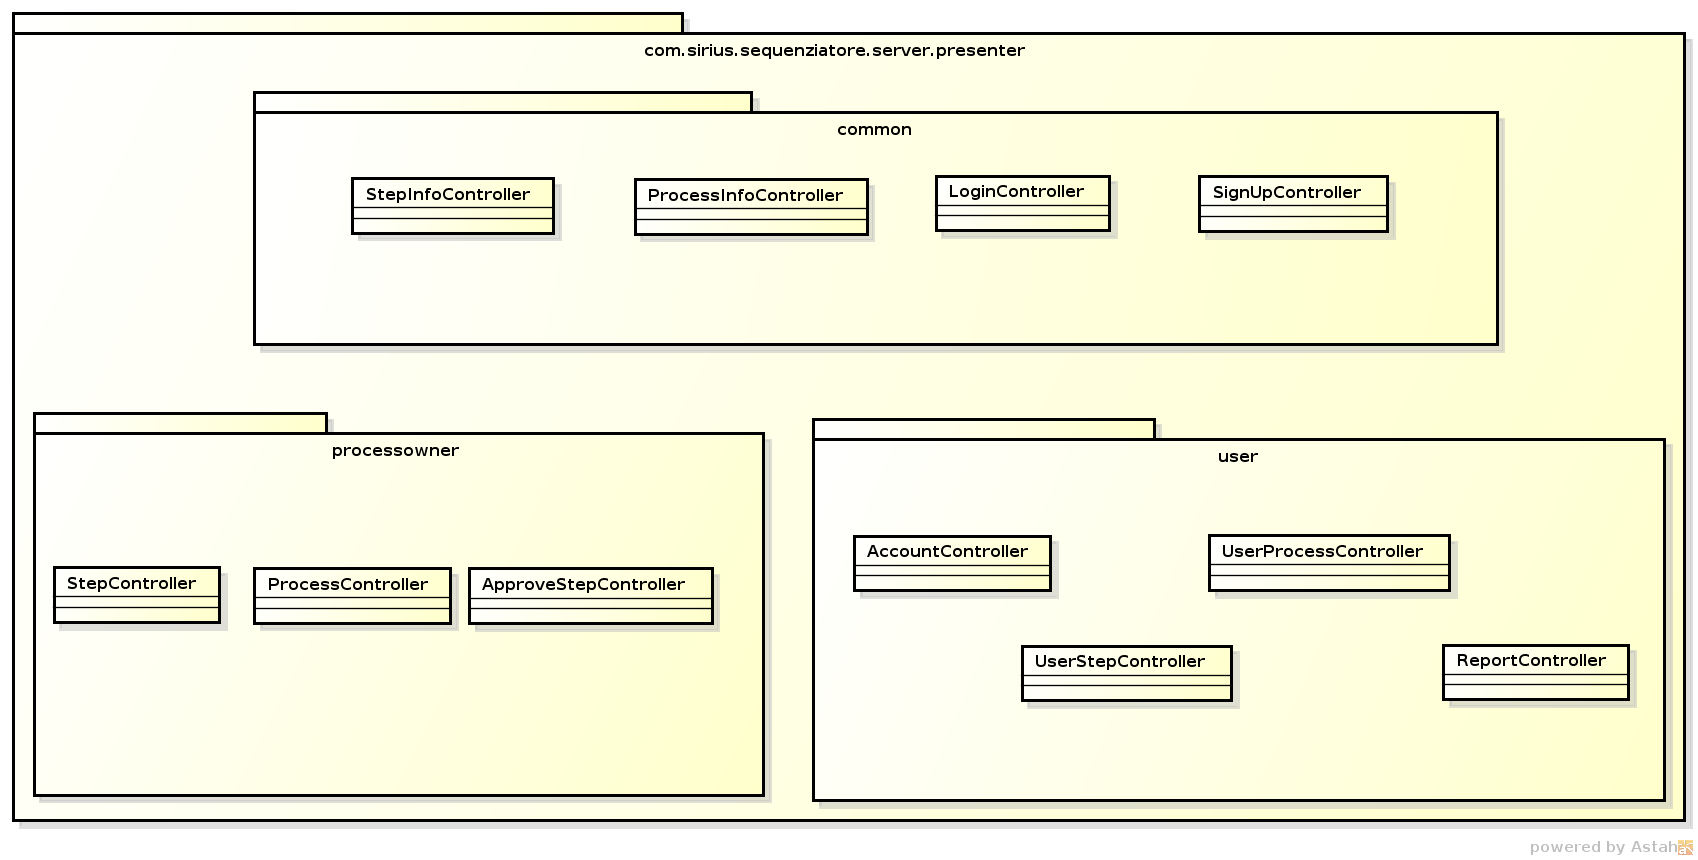
\includegraphics[width=%
\textwidth]
{./pack/ClassiServerSoloPresenter.png} \caption{Diagramma presenter server}
\end{figure}
\subsubsection{Package com.sirius.sequenziatore.server.presenter.common}
Questo \textit{package} contiene le classi che effettuano operazioni generali oppure comuni tra \textit{Process Owner} e Utenti.
\paragraph{LoginController}
	\begin{itemize}
		\item \textbf{Nome:} \texttt{LoginController};
		\item \textbf{Package:} com.sirius.sequenziatore.server.presenter.common
		\item \textbf{Descrizione:} Classe che permette la gestione della login di un utilizzatore del sistema, controllando che i dati inseriti riferiscano a un utente correttamente iscritto al sistema, ponendo attenzione se esso sia un \textit{process owner} o un utente normale;
		\item \textbf{Relazione con altre componenti:} la classe invoca i metodi della classe:
		\begin{itemize}
			\item com.sirius.sequenziatore.server.model.IDataAccessObject;
		\end{itemize}
	\end{itemize}
	
\paragraph{SignUpConroller}
	\begin{itemize}
		\item \textbf{Nome:} \texttt{SignUpController};
		\item \textbf{Package:} com.sirius.sequenziatore.server.presenter.common
		\item \textbf{Descrizione:} Classe che permette la gestione della registrazione di un nuovo utente nel sistema, nonostante la correttezza dei dati inseriti venga controllata dalla parte client, per sicurezza verrà effettuato un nuovo controllo anche sulla parte server prima di inserire un utente nel sistema;
		\item \textbf{Relazione con altre componenti:} la classe invoca i metodi della classe:
		\begin{itemize}
			\item com.sirius.sequenziatore.server.model.IDataAccessObject;
		\end{itemize}
	\end{itemize}
	
\paragraph{StepInfoController}
	\begin{itemize}
		\item \textbf{Nome:} \texttt{StepInfoController};
		\item \textbf{Package:} com.sirius.sequenziatore.server.presenter.common
		\item \textbf{Descrizione:} Classe che fornisce a chi lo richiede lo scheletro di un passo, quindi andrà a fornire i dati da inserire per tale passo e altre informazioni;
		\item \textbf{Relazione con altre componenti:} la classe invoca i metodi della classe:
		\begin{itemize}
			\item com.sirius.sequenziatore.server.model.IDataAccessObject;
		\end{itemize}
	\end{itemize}
\paragraph{ProcessInfoController}
	\begin{itemize}
		\item \textbf{Nome:} \texttt{ProcessInfoController};
		\item \textbf{Package:} com.sirius.sequenziatore.server.presenter.common
		\item \textbf{Descrizione:} Classe incaricata di fornire a chi lo richieda lo scheletro di un processo, come ad esempio numero di passi o condizioni per il suo completamento;
		\item \textbf{Relazione con altre componenti:} la classe invoca i metodi della classe:
		\begin{itemize}
			\item com.sirius.sequenziatore.server.model.IDataAccessObject;
		\end{itemize}
	\end{itemize}


\subsubsection{Package com.sirius.sequenziatore.server.presenter.user}
\paragraph{AccountController}
	\begin{itemize}
		\item \textbf{Nome:} \texttt{AccountController};
		\item \textbf{Package:} com.sirius.sequenziatore.server.presenter.user
		\item \textbf{Descrizione:} classe che permette la modifica dei dati di un utente come password o altre informazioni inerenti ai dettagli personali di un utente;
		\item \textbf{Relazione con altre componenti:} la classe richiama i metodi della classe:
		\begin{itemize}
			\item com.sirius.sequenziatore.server.model.IDataAccessObject;
		\end{itemize}
	\end{itemize}
%-----------------------------------------------------------------------------------------------%
\paragraph{UserProcessController}
	\begin{itemize}
		\item \textbf{Nome:} \texttt{UserProcessController};
		\item \textbf{Package:} com.sirius.sequenziatore.server.presenter.user
		\item \textbf{Descrizione:} classe che restituisce all' utente i dati di uno o più processi, può inoltre permettere l' inoltro della richiesta di un utente a iscriversi o disiscriversi a un processo;
		\item \textbf{Relazione con altre componenti:} la classe richiama i metodi della classe:
		\begin{itemize}
			\item com.sirius.sequenziatore.server.model.IDataAccessObject;
		\end{itemize}
	\end{itemize}
%-----------------------------------------------------------------------------------------------%
\paragraph{UserStepController}
	\begin{itemize}
		\item \textbf{Nome:} \texttt{UserStepController};
		\item \textbf{Package:} com.sirius.sequenziatore.server.presenter.user
		\item \textbf{Descrizione:} Gestisce l' esecuzione di un passo da parte di un utente inoltrando la richiesta di inserire i dati nel \textit{database} e in caso sia richiesto, notifica l' amministratore che deve controllare se il passo è stato completato, inoltre è incaricato di restituire i dati inseriti di un passo quando richiesto da un utente;
		\item \textbf{Relazione con altre componenti:} la classe richiama i metodi della classe:
		\begin{itemize}
			\item com.sirius.sequenziatore.server.model.IDataAccessObject;
		\end{itemize}
	\end{itemize}
%-----------------------------------------------------------------------------------------------%
\paragraph{ReportController}
	\begin{itemize}
		\item \textbf{Nome:} \texttt{ReportController};
		\item \textbf{Package:} com.sirius.sequenziatore.server.presenter.user
		\item \textbf{Descrizione:} Classe che fornisce i dati per generare il report dell' utente riferito al processo richiesto;
		\item \textbf{Relazione con altre componenti:} la classe implementa l' interfaccia sequenziatore.server.presenter.iuser.IReport e richiama i metodi della classe:
		\begin{itemize}
			\item com.sirius.sequenziatore.server.model.IDataAccessObject;
		\end{itemize}
	\end{itemize}
%-----------------------------------------------------------------------------------------------%%1
\subsubsection{Package sequenziatore::server::presenter::iprocessowner}
\paragraph{IProcessManager}
	\begin{itemize}
		\item \textbf{Nome:} \texttt{IProcessManager};
		\item \textbf{Package:} sequenziatore::server::presenter::iprocessowner
		\item \textbf{Descrizione:} Interfaccia che permette la gestione dei processi al \textit{process owner};
	\end{itemize}

%----------------------------------------------------------------------------------------------%

\paragraph{IStepManager}
	\begin{itemize}
		\item \textbf{Nome:} \texttt{IStepManager};
		\item \textbf{Package:} sequenziatore::server::presenter::iprocessowner
		\item \textbf{Descrizione:} Interfaccia che permette la gestione dei passi al \textit{process owner};
	\end{itemize}

%----------------------------------------------------------------------------------------------%
\paragraph{IUserManager}
	\begin{itemize}
		\item \textbf{Nome:} \texttt{IUserManager};
		\item \textbf{Package:} sequenziatore::server::presenter::iprocessowner
		\item \textbf{Descrizione:} Interfaccia per la gestione degli utenti iscritti ai processi;
	\end{itemize}
%----------------------------------------------------------------------------------------------%

\paragraph{IReport}
	\begin{itemize}
		\item \textbf{Nome:} \texttt{IReport};
		\item \textbf{Package:} sequenziatore::server::presenter::iprocessowner
		\item \textbf{Descrizione:} Interfaccia che permette la gestione dei report al \textit{process owner};
	\end{itemize}

%0000000000000000000000000000000000000000000000000000000000000000000000000000000000000000000000000%
\subsubsection{Package sequenziatore::server::presenter::processowner}

\paragraph{ProcessManager}
	\begin{itemize}
		\item \textbf{Nome:} \texttt{ProcessManager};
		\item \textbf{Package:} sequenziatore::server::presenter::processowner
		\item \textbf{Descrizione:} Classe che riceve le richieste del \textit{process owner} per la gestione dei processi come creazione,modifica e eliminazione degli stessi;
		\item \textbf{Relazione con altre componenti:} la classe implementa l' intefaccia sequenziatore::server::presenter::iprocessowner::IProcessManager ed invoca i metodi delle classi:
		\begin{itemize}
			\item \textcolor{red}{manca}
		\end{itemize}
	\end{itemize}
%----------------------------------------------------------------------------------------------%
\paragraph{StepManager}
	\begin{itemize}
		\item \textbf{Nome:} \texttt{StepManager};
		\item \textbf{Package:} sequenziatore::server::presenter::processowner
		\item \textbf{Descrizione:} Classe che permette l' elaborazione delle richieste del \textit{process owner} per quanto concerne la creazione,la rimozione e la modifica di passi;
		\item \textbf{Relazione con altre componenti:} la classe implementa l' intefaccia sequenziatore::server::presenter::iprocessowner::IStepManager ed invoca i metodi delle classi:
		\begin{itemize}
			\item \textcolor{red}{manca}
		\end{itemize}
	\end{itemize}
	%----------------------------------------------------------------------------------------------%
\paragraph{UserManager}
	\begin{itemize}
		\item \textbf{Nome:} \texttt{UserManager};
		\item \textbf{Package:} sequenziatore::server::presenter::iprocessowner
		\item \textbf{Descrizione:} Classe che permette la gestione degli utenti iscritti alla piattaforma, permettendogli di rimuovere utenti da processi,;
		\item \textbf{Relazione con altre componenti:} la classe implementa l' intefaccia sequenziatore::server::presenter::iprocessowner::IUserManager ed invoca i metodi delle classi:
		\begin{itemize}
			\item \textcolor{red}{manca}
		\end{itemize}
	\end{itemize}

%----------------------------------------------------------------------------------------------%
\paragraph{Report}
	\begin{itemize}
		\item \textbf{Nome:} \texttt{Report};
		\item \textbf{Package:} sequenziatore::server::presenter::iprocessowner
		\item \textbf{Descrizione:} Classe che permette la gestione delle richieste dei report al \textit{process owner}, permettendogli di visualizzare i risultati raggiunti in un processo;
		\item \textbf{Relazione con altre componenti:} la classe implementa l' intefaccia sequenziatore::server::presenter::iprocessowner::IReport ed invoca i metodi delle classi:
		\begin{itemize}
			\item \textcolor{red}{manca}
		\end{itemize}
	\end{itemize}
%2
\subsection{Package sequenziatore::server::model}
\paragraph{DaoFacade}
	\begin{itemize}
		\item \textbf{Nome:} \texttt{DaoFacade};
		\item \textbf{Tipo:} abstract;
		\item \textbf{Package:} sequenziatore::server::model
		\item \textbf{Descrizione:} Classe astratta che decide a che pacchetto assegnare la richiesta di esecuzione \textit{query};
		\item \textbf{Relazione con altre componenti:} la classe invoca i metodi delle seguenti classi:
		\begin{itemize}
			\item sequenziatore::server::model::daoprocessowner::ObjectTransfer tramite l' interfaccia sequenziatore::server::model::daoprocessowner::IObjectTransfer
			\item sequenziatore::server::model::daoprocessowner::DataAccessObject tramite l' interfaccia sequenziatore::server::model::daoprocessowner::IDataAccessObject
			\item sequenziatore::server::model::daostep::ObjectTransfer tramite l' interfaccia sequenziatore::server::model::daostep::IObjectTransfer
			\item sequenziatore::server::model::daostep::DataAccessObject tramite l' interfaccia sequenziatore::server::model::daostep::IDataAccessObject
			\item sequenziatore::server::model::daouser::ObjectTransfer tramite l' interfaccia sequenziatore::server::model::daouser::IObjectTransfer
			\item sequenziatore::server::model::daouser::DataAccessObject tramite l' interfaccia sequenziatore::server::model::daouser::IDataAccessObject
			\item sequenziatore::server::model::daoprocess::ObjectTransfer tramite l' interfaccia sequenziatore::server::model::daoprocess::IObjectTransfer
			\item sequenziatore::server::model::daoprocess::DataAccessObject tramite l' interfaccia sequenziatore::server::model::daoprocess::IDataAccessObject
		\end{itemize}
	\end{itemize}
\subsubsection{Package sequenziatore::server::model::daouser}
\paragraph{IDataAccessObject}
	\begin{itemize}
		\item \textbf{Nome:} \texttt{IDataAccessObject};
		\item \textbf{Package:} sequenziatore::server::model::daouser
		\item \textbf{Descrizione:} Interfaccia con il compito di interagire con il database.
	\end{itemize}
%------------------------------------------------------------------------------%
\paragraph{DataAccessObject}
	\begin{itemize}
		\item \textbf{Nome:} \texttt{DataAccessObject};
		\item \textbf{Package:} sequenziatore::server::model::daouser
		\item \textbf{Descrizione:} classe che si occupa di effettuare le richieste al database, acquisendo i dati richiesti o inserendone di nuovi.
		\item \textbf{Relazione con altre componenti:} la classe implementa l' interfaccia sequenziatore::server::model::daouser::IDataAccessObject ed invoca metodi delle classi:
		\begin{itemize}
			\item sequenziatore::server::model::daouser::ObjectTransfer tramite l' interfaccia sequenziatore::server::model::daouser::IObjectTransfer
		\end{itemize}
	\end{itemize}
	%------------------------------------------------------------------------------%
\paragraph{IObjectTransfer}
	\begin{itemize}
		\item \textbf{Nome:} \texttt{IObjectTransfer};
		\item \textbf{Package:} sequenziatore::server::model::daouser
		\item \textbf{Descrizione:} Interfaccia che permette lo scambio di dati tra model e presenter.
	\end{itemize}
	%------------------------------------------------------------------------------%
\paragraph{ObjectTransfer}
	\begin{itemize}
		\item \textbf{Nome:} \texttt{ObjectTransfer};
		\item \textbf{Package:} sequenziatore::server::model::daouser
		\item \textbf{Descrizione:} Classe che permette lo scambio di dati tra la classe DataAccessObject e il presenter.
		\item \textbf{Relazione con altre componenti:} la classe implementa l'interfaccia sequenziatore::server::model::daouser::IObjectTransfer.
	\end{itemize}
%000000000000000000000000000000000000000000000000000000000000000000000000000000000000%
\subsubsection{Package sequenziatore::server::model::daoprocessowner}
\paragraph{IDataAccessObject}
	\begin{itemize}
		\item \textbf{Nome:} \texttt{IDataAccessObject};
		\item \textbf{Package:} sequenziatore::server::model::daoprocessowner
		\item \textbf{Descrizione:} Interfaccia con il compito di interagire con il database.
	\end{itemize}
	%------------------------------------------------------------------------------%
\paragraph{DataAccessObject}
\begin{itemize}
		\item \textbf{Nome:} \texttt{DataAccessObject};
		\item \textbf{Package:} sequenziatore::server::model::daoprocessowner
		\item \textbf{Descrizione:} classe che si occupa di effettuare le richieste al database, acquisendo i dati richiesti o inserendone di nuovi.
		\item \textbf{Relazione con altre componenti:} la classe implementa l' interfaccia sequenziatore::server::model::daoprocessowner::IDataAccessObject ed invoca metodi delle classi:
		\begin{itemize}
			\item sequenziatore::server::model::daoprocessowner::ObjectTransfer tramite l' interfaccia sequenziatore::server::model::daoprocessowner::IObjectTransfer
		\end{itemize}
\end{itemize}
	%------------------------------------------------------------------------------%
\paragraph{IObjectTransfer}
	\begin{itemize}
		\item \textbf{Nome:} \texttt{IObjectTransfer};
		\item \textbf{Package:} sequenziatore::server::model::daoprocessowner
		\item \textbf{Descrizione:} Interfaccia che permette lo scambio di dati tra model e presenter.
	\end{itemize}
	%------------------------------------------------------------------------------%
\paragraph{ObjectTransfer}
	\begin{itemize}
		\item \textbf{Nome:} \texttt{ObjectTransfer};
		\item \textbf{Package:} sequenziatore::server::model::daoprocessowner
		\item \textbf{Descrizione:} Classe che permette lo scambio di dati tra la classe DataAccessObject e il presenter.
		\item \textbf{Relazione con altre componenti:} la classe implementa l'interfaccia sequenziatore::server::model::daoprocessowner::IObjectTransfer.
	\end{itemize}
%000000000000000000000000000000000000000000000000000000000000000000000000000000000000%
\subsubsection{Package sequenziatore::server::model::daoprocess}
\paragraph{IDataAccessObject}
	\begin{itemize}
		\item \textbf{Nome:} \texttt{IDataAccessObject};
		\item \textbf{Package:}sequenziatore::server::model::daoprocess
		\item \textbf{Descrizione:} Interfaccia con il compito di interagire con il database.
	\end{itemize}
	%------------------------------------------------------------------------------%
\paragraph{DataAccessObject}
	\begin{itemize}
		\item \textbf{Nome:} \texttt{DataAccessObject};
		\item \textbf{Package:} sequenziatore::server::model::daoprocess
		\item \textbf{Descrizione:} classe che si occupa di effettuare le richieste al database, acquisendo i dati richiesti o inserendone di nuovi.
		\item \textbf{Relazione con altre componenti:} la classe implementa l' interfaccia sequenziatore::server::model::daoprocess::IDataAccessObject ed invoca metodi delle classi:
		\begin{itemize}
			\item sequenziatore::server::model::daoprocess::ObjectTransfer tramite l' interfaccia sequenziatore::server::model::daoprocess::IObjectTransfer
	\end{itemize}
\end{itemize}
	%------------------------------------------------------------------------------%
\paragraph{IObjectTransfer}
	\begin{itemize}
		\item \textbf{Nome:} \texttt{IObjectTransfer};
		\item \textbf{Package:} sequenziatore::server::model::daoprocess
		\item \textbf{Descrizione:} Interfaccia che permette lo scambio di dati tra model e presenter.
	\end{itemize}
	%------------------------------------------------------------------------------%
\paragraph{ObjectTransfer}
	\begin{itemize}
		\item \textbf{Nome:} \texttt{ObjectTransfer};
		\item \textbf{Package:} sequenziatore::server::model::daoprocess
		\item \textbf{Descrizione:} Classe che permette lo scambio di dati tra la classe DataAccessObject e il presenter.
		\item \textbf{Relazione con altre componenti:} la classe implementa l'interfaccia sequenziatore::server::model::daoprocess::IObjectTransfer.
	\end{itemize}
%000000000000000000000000000000000000000000000000000000000000000000000000000000000000%
\subsubsection{Package sequenziatore::server::model::daostep}
\paragraph{IDataAccessObject}
	\begin{itemize}
		\item \textbf{Nome:} \texttt{IDataAccessObject};
		\item \textbf{Package:} sequenziatore::server::model::daostep
		\item \textbf{Descrizione:} Interfaccia con il compito di interagire con il database.
	\end{itemize}
	%------------------------------------------------------------------------------%
\paragraph{DataAccessObject}
	\begin{itemize}
		\item \textbf{Nome:} \texttt{DataAccessObject};
		\item \textbf{Package:} sequenziatore::server::model::daostep
		\item \textbf{Descrizione:} classe che si occupa di effettuare le richieste al database, acquisendo i dati richiesti o inserendone di nuovi.
		\item \textbf{Relazione con altre componenti:} la classe implementa l' interfaccia sequenziatore::server::model::daostep::IDataAccessObject ed invoca metodi delle classi:
		\begin{itemize}
			\item sequenziatore::server::model::daostep::ObjectTransfer tramite l' interfaccia sequenziatore::server::model::daostep::IObjectTransfer
	\end{itemize}
	\end{itemize}
	%------------------------------------------------------------------------------%
\paragraph{IObjectTransfer}
	\begin{itemize}
		\item \textbf{Nome:} \texttt{IObjectTransfer};
		\item \textbf{Package:} sequenziatore::server::model::daostep
		\item \textbf{Descrizione:} Interfaccia che permette lo scambio di dati tra model e presenter.
	\end{itemize}
	%------------------------------------------------------------------------------%
\paragraph{ObjectTransfer}
	\begin{itemize}
		\item \textbf{Nome:} \texttt{ObjectTransfer};
		\item \textbf{Package:} sequenziatore::server::model::daostep
		\item \textbf{Descrizione:} Classe che permette lo scambio di dati tra la classe DataAccessObject e il presenter.
		\item \textbf{Relazione con altre componenti:} la classe implementa l'interfaccia sequenziatore::server::model::daostep::IObjectTransfer.
	\end{itemize}
\section{Design pattern}

\subsection{Design pattern architetturali}

\subsubsection{Model View Presenter}
\begin{itemize}
\item \textbf{Scopo:}
Il \textit{pattern\ped{G}} architetturale \textit{Model View Presenter} (MVP) è un derivato del \textit{Model View Controller} (MVC), focalizzato sulla valorizzazione della logica della presentazione. Entrambi i pattern hanno lo sopo di disaccoppiare la logica dell'applicazione dalla rappresentazione grafica.\\
Il \textit{pattern\ped{G}} MVP prevede la suddivisione dell'applicazione in tre componenti:
\begin{itemize}
\item \textbf{Model:} Definisce il modello dati e le regole di accesso e di modifica;
\item \textbf{View:} Si occupa della rappresentazione dell'interfaccia utente;
\item \textbf{Presenter:} Contiene la logica dell'applicazione, si occupa delle comunicazioni tra vista e modello e dell'aggiornamento della vista.
\end{itemize}

\item \textbf{Contesto d'uso:}
\end{itemize}

\subsection{Design pattern strutturali}
\subsubsection{Adapter}
\begin{itemize}
\item \textbf{Scopo:}
Il \textit{pattern\ped{G}} strutturale \textit{Adapter} permette di utilizzare un componente software la cui interfaccia deve essere adattata per potersi integrare ad un'altra presente nell'applicazione esistente.\\
Tale \textit{pattern\ped{G}} può essere basato sia su classi che su oggetti, perciò, l'istanza della classe da adattare, può derivare tramite ereditarietà o composizione.

\item \textbf{Contesto d'uso:}
\end{itemize}

\subsubsection{Decorator}
\begin{itemize}
\item \textbf{Scopo:}
Il \textit{pattern\ped{G}} strutturale \textit{Decorator} permette di aggiungere dinamicamente funzionalità ad un oggetto base, con la possibilità di comporle arbitrariamente.\\
Tale \textit{pattern\ped{G}} si pone come alternativa all'uso dell'ereditarietà singola o multipla;

\item \textbf{Contesto d'uso:}
\end{itemize}

\subsubsection{Facade}
\begin{itemize}
\item \textbf{Scopo:}
Il \textit{pattern\ped{G}} strutturale \textit{Facade} prevede l'utilizzo di un'interfaccia unica e semplice per un sottosistema complesso, diminuendo la complessità del sistema;

\item \textbf{Contesto d'uso:}
\end{itemize}

\subsubsection{Proxy}
\begin{itemize}
\item \textbf{Scopo:}
Il \textit{pattern\ped{G}} strutturale \textit{Proxy} viene utilizzato per accedere ad un un oggetto complesso di cui si vogliono controllare gli accessi, tramite un oggetto semplice, che espone gli stessi metodi dell'oggetto che maschera;

\item \textbf{Contesto d'uso:}
\end{itemize}

\subsection{Design pattern creazionali}
\subsubsection{Singleton}
\begin{itemize}
\item \textbf{Scopo:}
Il \textit{pattern\ped{G}} creazionale \textit{Singleton} viene utilizzato quando si ha la necessità di avere una sola istanza di una classe e di avere un punto di accesso globale ad essa;

\item \textbf{Contesto d'uso:}
\end{itemize}

\subsubsection{Abstract Factory}
\begin{itemize}
\item \textbf{Scopo:}
Il \textit{pattern\ped{G}} creazionale \textit{Abstract Factory} fornisce un'interfaccia per creare famiglie di prodotti senza specificare classi concrete. Le classi che concretizzano tale interfaccia, vengono costruite una sola volta, e consentono di utilizzare una varietà di elementi che presentano le stesse funzionalità con diverse implementazioni;

\item \textbf{Contesto d'uso:}
\end{itemize}

\subsection{Design pattern comportamentali}
\subsubsection{Command}
\begin{itemize}
\item \textbf{Scopo:}
Il \textit{pattern\ped{G}} comportamentale \textit{Command} permette di separare l'invocazione di un comando dai suoi dettagli implementativi;

\item \textbf{Contesto d'uso:}
\end{itemize}

\subsubsection{Iterator}
\begin{itemize}
\item \textbf{Scopo:}
Il \textit{pattern\ped{G}} comportamentale \textit{Iterator} fornisce l'accesso sequenziale agli elementi di un aggregato senza esporne l'implementazione;

\item \textbf{Contesto d'uso:}
\end{itemize}

\subsubsection{Observer}
\begin{itemize}
\item \textbf{Scopo:}
Il \textit{pattern\ped{G}} comportamentale \textit{Observer} viene utilizzato quando si vuole realizzare una dipendenza tra un soggetto e più oggetti, in cui il cambiamento di stato del un soggetto, viene notificato a tutti gli oggetti dipendenti;

\item \textbf{Contesto d'uso:}
\end{itemize}

\subsubsection{Strategy}
\begin{itemize}
\item \textbf{Scopo:}
Il \textit{pattern\ped{G}} comportamentale \textit{Strategy} viene utilizzato per definire una famiglia di algoritmi, incapsularli e renderli intercambiabili;

\item \textbf{Contesto d'uso:}
\end{itemize}

\subsubsection{Template method}
\begin{itemize}
\item \textbf{Scopo:}
Il \textit{pattern\ped{G}} comportamentale \textit{Template method} viene utilizzato per definire lo scheletro di un algoritmo, lasciando l'implementazione di alcuni passi alle sottoclassi. In particolare consente di specificare l'ordine delle operazioni da effettuare ma di delegare la loro implementazione o parte di essa alle sottoclassi;

\item \textbf{Contesto d'uso:}
\end{itemize}
\section{Diagrammi di attività}
Di seguito vengono illustrati i diagrammi di attività che illustrano l'interazione degli utenti con il l'applicativo \progetto{}.
Si è cercato di creare diagrammi ad alto livello che descrivessero il principale flusso di azioni. Tali diagrammi sono in seguito stati suddivisi secondo sotto-diagrammi specifici, al fine di illustrare con maggior dettaglio il flusso di certe attività.

\subsection{Diagrammi di attività: process owner}

\subsubsection{Creazione processo}
\begin{figure}[H]
\centering
\includegraphics[trim=0cm 0.8cm 0cm 0cm,clip=true,scale=0.50]%
{./attivita/admin/creazioneprocesso}
\caption{Attività process owner: creazione processo.}
\end{figure}

\textbf{Descrizione}: Il process owner\ped{G} al fine di creare un nuovo processo dovrà dapprima inserire il nome e la descrizione del suddetto. Inseriti i primi campi potrà inserire
o una data di scadenza o un numero massimo di completamenti del processo, alchè sarà tenuto a definire i passi del suddetto (per maggiori dettagli vedere: Figura 3, Attività process owner: creazione passo). Eseguiti i passi sopracitati potrà decidere se annullare il processo o darne la conferma
\subsubsection{Gestione processo}
\begin{figure}[H]
\centering
\includegraphics[trim=0cm 0.8cm 0cm 0cm,clip=true,scale=0.40]%
{./attivita/admin/gestioneprocesso}
\caption{Attività process owner: gestione di un processo.}
\end{figure}

\textbf{Descrizione}: Brevemente il process owner dopo aver visualizzato la lista processi, può selezionare il processo di interesse per accedere alla sua gestione, ossia: visualizzare utenti (al fine di aggiungerli al processo), eliminare il processo, terminarlo oppure recuperare le informazioni relative al suddetto.
Il recupero delle informazioni è necessario per controllare i dati che richiedono la verifica umana. Nel momento in cui il process owner ha finito di gestire i processi, potrà chiudere l'applicazione.

\subsubsection{Creazione passo}
\begin{figure}[H]
\centering
\includegraphics[trim=0cm 0.8cm 0cm 0cm,clip=true,scale=0.50]%
{./attivita/admin/creazionepasso}
\caption{Attività process owner: creazione passo.}
\end{figure}

\textbf{Descrizione}: durante la creazione /modifica di un processo l'utente process owner potrà decidere di aggiungere dei passi, l'aggiunta di un passo comporta l'aggiunta dei dati che gli competono, che possono essere di tre tipologie. Compiuta l'aggiunta dei dati, sarà possibile imporre dei vincoli su questi dati, al fine di determinare se l'utente gli ha inseriti rispettandoli. In questa fase è inoltre possibile inserire un vincolo geografico (coordinate GPS). Attuato questo flusso di comandi il passo potrà essere avviato oppure annullato a discrezione del process owner.

\subsubsection{Gestione passi}
\begin{figure}[H]
\centering
\includegraphics[trim=0cm 0.8cm 0cm 0cm,clip=true,scale=0.40]%
{./attivita/admin/definizionepasso}
\caption{Attività process owner: gestione passi.}
\end{figure}

\textbf{Descrizione}: La gestione dei passi di un processo si dirama in 4 possibili scelte: la creazione di un nuovo passo, la modifica di un passo esistente, l'eliminazione di un passo e la visualizzazione dei passi creati. Per quanto concerne la modifica e l'eliminazione di un passo l'utente potrà scegliere se annullare o apportare effettivamente le modifiche/eliminazione.

\subsection{Diagrammi di attività: standard user}

\subsubsection{Registrazione}
\begin{figure}[H]
\centering
\includegraphics[trim=0cm 0.8cm 0cm 0cm,clip=true,scale=0.50]%
{./attivita/user/Registrazione}
\caption{Attività user: Registrazione}
\end{figure}

\textbf{Descrizione}: L'utente inserisce i dati richiesti per la registrazione, se  l'username scelto è unico, allora i dati vengono salvati, l'utente è registrato e può autenticarsi, in caso contrario viene richiesto di inserire un nuovo username.


\subsubsection{Login}
\begin{figure}[H]
\centering
\includegraphics[trim=0cm 0.8cm 0cm 0cm,clip=true,scale=0.50]%
{./attivita/user/Login}
\caption{Attività user: Login}
\end{figure}

\textbf{Descrizione}: L'utente non autenticato inserisce i suoi dati d'accesso, se sono corretti, l'utente viene autenticato, altrimenti gli viene notificato l'errore.

\subsubsection{Modifica dati utente}
\begin{figure}[H]
\centering
\includegraphics[trim=0cm 0.8cm 0cm 0cm,clip=true,scale=0.50]%
{./attivita/user/Modificautente}
\caption{Attività user: Modifica dati utente}
\end{figure}

\textbf{Descrizione}: I dati che l'utente può modificare una volta reistrato sono la sua password e la sua email.
Se l'utente vuole modificare la password gli viene priam richiesta la password corrente, se non è corretta gli viene notificato un errore e la richiesta viene ripetuta, in caso contrario l'utente inserisce una nuova password.
Se invece l'utente vuole modificare la sua email, gli viene semplicemnte richiesta una nuova mail.
In caso di modifica di password o email i dai vengono risalvati sul server.

\subsubsection{Gestione dei processi}
\begin{figure}[H]
\centering
\includegraphics[trim=0cm 0.8cm 0cm 0cm,clip=true,scale=0.50]%
{./attivita/user/Gestioneprocessi}
\caption{Attività user: Gestione dei processi}
\end{figure}

\textbf{Descrizione}: Il sistema dopo aver ricevuto dal server i dati sui processi che l'utente può gestire, ne visualizza una lista, l'utente seleziona un processo dalla lista di cui riceve successivamente la descrizione.
Se l'utente è iscritto al processo selezionato può eseguire il processo e/o pùò disiscriversi da questo processo.
Se non è iscritto invece può decidere di iscriversi, e una volta iscritto gli vengono offerte le stesse attività descritte nel caso precedente.

\subsubsection{Esecuzione di un processo}
\begin{figure}[H]
\centering
\includegraphics[trim=0cm 0.8cm 0cm 0cm,clip=true,scale=0.50]%
{./attivita/user/Esecuzioneprocesso}
\caption{Attività user: Esecuzione di un processo}
\end{figure}

\textbf{Descrizione}: All'utente vengono visualizzate le informazioni sul processo in esecuzione, dopodichè, per ogni passo del processo, l'utente segue il passo (si veda il diagramma delle attività "Esecuzione di un passo" per i dettagli), e il sistema determina il passo succesivo.
Infine, al terminie dei passi che il sistema ha determinato da eseguire, il processo viene concluso (si veda il digramma delle attività "Conclusione di un processo" per i dettagli).


\subsubsection{Conclusione di un processo}
\begin{figure}[H]
\centering
\includegraphics[trim=0cm 0.8cm 0cm 0cm,clip=true,scale=0.50]%
{./attivita/user/Conclusioneprocesso}
\caption{Attività user: conclusione di un processo}
\end{figure}

\textbf{Descrizione}: Il sistema genera un report sui passi eseguiti e sui dati raccolti, questo report viene inviato al server.
Successivamente l'utente può scegliere se visualizzare il report e se salvarne una copia sul proprio dispositivo.
Infine il processo viene chiuso.

\subsubsection{Esecuzione di un passo}
\begin{figure}[H]
\centering
\includegraphics[trim=0cm 0.8cm 0cm 0cm,clip=true,scale=0.50]%
{./attivita/user/Esecuzionepasso}
\caption{Attività user: Esecuzione di un passo}
\end{figure}

\textbf{Descrizione}: All'utente vengono visualizzate le informazioni sul passo, poi se il passo è opzionale l'utente può decidere di saltarlo.
Nel caso il passo non sia opzionale o che l'utente non voglia saltarlo, l'utente inserisce i dati richisti per il completamento del passo, i quali vengono successivamente inviati al server.
Se i dati inviati richiedono il controllo dell'amministratore, il passo non può essere completato fino alla ricezione del suo giudizio che può richiedere di ripetere l'esecuzione del passo.
Nel caso che i dati soddisfino il l'amministratore o non fosse richiesto il controllo, il passo viene concluso.



\section{Tracciamento}

\subsection{Tracciamento package - componenti}
\LTXtable{0.9\textwidth}{Package-Componenti.tex}
\subsection{Tracciamento componenti - requisiti}
\LTXtable{\textwidth}{Componenti-Requisiti.tex}
\subsection{Tracciamento requisiti - componenti}
\LTXtable{\textwidth}{Requisiti-Componenti.tex}
\appendix
\section{Tecnologie utilizzate}
\subsection{Spring Framework}
Spring è stato scelto per rendere più facile lo sviluppo della nostra applicazione lato server, infatti non è necessario configurare e realizzare le servlet perchè vengono automaticamente gestite e realizzate dal framework. Inoltre rende facile e chiara la separazione delle componenti grazie al suo sistema di annotazioni e anche un codice più pulito, come nel caso di @RequestBody, che grazie alla libreria JacksonJson trasforma automaticamente l' oggetto JSON ricevuto dal controller nell' oggetto Java voluto.
\subsection{HTML5}
\textit{HTML5\ped{G}}, richiesto espressamente dal proponente all'interno del capitolato d'appalto, verrà utilizzato per la struttura base della pagine, inoltre ci permetterà di utilizzare il controllo della geolocalizzazione, fondamentale nello sviluppo del nostro sistema, oltre alle altre novità che introduce.
\subsection{CSS3}
\textit{CSS3} è un linguaggio \textit{style sheet} verrà utilizzato per la rappresentazione grafica delle pagine, in modo da separarla dai contenuti. In questo modo verranno migliorate comprensione, manutenibilità e portabilità.
\subsection{Javascript}
L' utilizzo di \textit{Javascript\ped{G}} è stato richiesto espressamente dal proponente, è un linguaggio di \textit{scripting} non compilato ma interpretato direttamente dal \textit{browser\ped{G}}. Nello sviluppo del nostro progetto ci permetterà di sviluppare l'applicazione lato lato \textit{client\ped{G}} e di comunicare con il \textit{server\ped{G}}.
\subsection{Backbone.js}
\textit{Backbone.js} è un \textit{framework} basato sul paradigma \textit{model-view-presenter}, utilizzata per lo sviluppo dell'applicazione \progetto{}.
Il \textit{framework} è particolarmente leggero e necessita come unica dipendenza della libreria \textit{Underscore.js}.
\textit{Backbone.js} è creato per sviluppare applicazioni \textit{web} di tipo \textit{single page}, e consente di strutturare il codice, grazie alle classi \textit{Model, View} e \textit{Router} estendibili dal programmatore.
Il gruppo \gruppo{} ha scelto questo \textit{framework}, in quanto si presta alle esigenze architetturali del progetto, e inoltre è molto ben documentato.
\subsection{Underscore.js}
\textit{Underscore.js} è una libreria necessaria al \textit{framework Backbone.js}. Viene utilizzata in particolare per gestire la comunicazione tra \textit{Backbone} e i \textit{template} utilizzati nel \textit{package view}.
\subsection{Require.js}
\textit{Require.js} è una libreria utilizzata per gestire le dipendenze tra le componenti e le librerie, e per implementare il \textit{pattern Asynchronous Module Definition
}. La libreria è stata scelta per l'ottima compatibilità con il \textit{framework Backbone.js}.
\subsection{JQuery}
\textit{Jquery} è una libreria \textit{Javascript} per applicazioni web.
La libreria consente di interagire con gli elementi \textit{DOM}, di gestire eventi e implementare funzionalità \textit{AJAX}.
\subsection{JQueryMobile}
Questa libreria verrà usata per lo sviluppo di un \textit{front-end} per dispositivi di tipo \textit{responsive}, accessibili da \textit{smartphne}, \textit{tablet} e computer. La scelta del team di questa libreria è data dal fatto che è affermata nel mondo del \textit{web development}.
\subsection{JAVA 7}
\textit{Java\ped{G}} è un linguaggio orientato agli oggetti che permette di essere quanto più indipendenti possibili dalla piattaforma di esecuzione. Nello sviluppo del nostro sistema verrà utilizzato nella la creazione del \textit{back-end}, in particolare per la creazione delle \textit{Servlet}.
\subsection{JSON}
\textit{JavaScript Object Notation} è il formato scelto per lo scambio dati tra \textit{client\ped{G}} e \textit{server\ped{G}}, è molto facile da utilizzare e si integra bene con la programmazione in AJAX e il suo uso con \textit{Javascript}. Il \textit{parsing} di tale tipo di dato viene effettuato con la semplice chiamata ad un metodo.
\subsection{JDBC}
\textit{Java DataBase Connectivity} è un connettore per \textit{database} in grado di consentire l'accesso alle basi di dati da un programma scritto in \textit{Java}. Fornisce i metodi per interrogare e modificare i dati nella base di dati.
\subsection{MySQL}
\textit{MySQL\ped{G}} è un Relational database management system(RDBMS). Il team ha scelto questo tipo di base di dati in quanto di semplice utilizzo e già utilizzata da tutti i membri del gruppo.
\subsection{Apache Tomcat}
\textit{Apache Tomcat} è un contenitore \textit{servlet} \textit{open source} che offre una piattaforma per l'esecuzione di applicazioni web sviluppate in \textit{Java}. La versione 4.x comprende \textit{Catalina} e \textit{Coyote}, rispettivamente il contenitore \textit{servlet} e il connettore \textit{HTTP}.

\end{document}